%%%%%%%%%%%%%%%%%%%%%%
\documentclass{singlecol-new}
%%%%%%%%%%%%%%%%%%%%%%

\usepackage{natbib,stfloats}
\usepackage{mathrsfs}

\def\newblock{\hskip .11em plus .33em minus .07em}

\theoremstyle{TH}{
\newtheorem{lemma}{Lemma}
\newtheorem{theorem}[lemma]{Theorem}
\newtheorem{corrolary}[lemma]{Corrolary}
\newtheorem{conjecture}[lemma]{Conjecture}
\newtheorem{proposition}[lemma]{Proposition}
\newtheorem{claim}[lemma]{Claim}
\newtheorem{stheorem}[lemma]{Wrong Theorem}
\newtheorem{algorithm}{Algorithm}
}

\theoremstyle{THrm}{
\newtheorem{definition}{Definition}[section]
\newtheorem{question}{Question}[section]
\newtheorem{remark}{Remark}
\newtheorem{scheme}{Scheme}
\newtheorem{example}{Example}
}

\theoremstyle{THhit}{
\newtheorem{case}{Case}[section]
}

%%%% Our commands %%%%

\usepackage{xspace}
\usepackage{paralist} % for compact lists: compactitem, compactenum, compactdesc
\usepackage{graphicx}
\usepackage{subfigure}

\newcommand{\pisodm}[0]{$\pi$SOD-M\xspace}
\def\FlyingPig{\textsl{FlyingPig}\xspace}


\makeatletter
\def\theequation{\arabic{equation}}

%\JOURNALNAME{\TEN{\it Int. J. System Control and Information
%Processing,
%Vol. \theVOL, No. \theISSUE, \thePUBYEAR\hfill\thepage}}%
%
%\def\BottomCatch{%
%\vskip -10pt
%\thispagestyle{empty}%
%\begin{table}[b]%
%\NINE\begin{tabular*}{\textwidth}{@{\extracolsep{\fill}}lcr@{}}%
%\\[-12pt]
%Copyright \copyright\ 2012 Inderscience Enterprises Ltd. & &%
%\end{tabular*}%
%\vskip -30pt%
%%%\vskip -35pt%
%\end{table}%
%}
\makeatother

%%%%%%%%%%%%%%%%%
\begin{document}%
%%%%%%%%%%%%%%%%%

\setcounter{page}{1}

\LRH{K. Belhajjame et~al.}

\RRH{\pisodm: Building SOC Applications in the Presence of Non-Functional Requirements}

\VOL{x}

\ISSUE{x}

\PUBYEAR{xxxx}

\BottomCatch

%\CLline

\PUBYEAR{2016}

\subtitle{}

\title{\pisodm: Building SOC Applications in the Presence of Non-Functional Requirements}

%
\authorA{Khalid Belhajjame}
%
\affA{Universit\'e de Paris - Dauphine -- Paris, France\\
  E-mail: kbelhajj@googlemail.com}
%
%
\authorB{Valeria~de~Castro}
\affB{Universidad Rey Juan Carlos -- M\'{o}stoles, Spain\\
  E-mail: valeria.decastro@urjc.es}
\authorC{Umberto~Souza~da~Costa}
\affC{Universidade Federal do Rio Grande do Norte -- Natal, Brazil\\
  E-mail: umberto@dimap.ufrn.br}

\authorD{Javier~A.~Espinosa-Oviedo}
\affD{Universidad de las Am\'ericas-Puebla, LAFMIA -- Cholula, Mexico\\
  E-mail: javiera.espinosa@gmail.com}
    
\authorE{Martin~A.~Musicante}
\affE{Universidade Federal do Rio Grande do Norte -- Natal, Brazil\\
  E-mail: mam@dimap.ufrn.br}

\authorF{Pl\'acido~A.~Souza~Neto}
\affF{Instituto Federal de Educa\c{c}\~{a}o, Ci\^{e}ncia e Tecnologia do Rio Grande do Norte -- Natal, Brazil\\
  E-mail: placido.neto@ifrn.edu.br}  

\authorG{Genoveva~Vargas-Solar}
\affG{CNRS, LIG-LAFMIA, Saint Martin d'H\`eres, France\\
  E-mail: genoveva.vargas@imag.fr}  

\authorH{Jos\'e-Luis~Zechinelli-Martini}
\affH{Universidad de las Am\'ericas-Puebla, LAFMIA -- Cholula, Mexico\\
  E-mail: joseluis.zechinelli@udlap.mx}


%
%\authorA{Fusheng Wang\footnote{Work done while working at Siemens Corporate Research.} }
%
%\affA{Department of Biomedical Informatics, Emory University
%\newline
%36 Eagle Row, Ste 589, Atlanta, GA 30322, USA}
%
%
%
%\authorB{\footnotesize Cristobal Vergara-Niedermayr\footnote{Work done while working at Siemens Corporate Research.}}
%\affB{Oracle \newline
 %New Jersey, USA}
%
%

\begin{abstract}
Specifying non-functional requirements (NFRs) is a complex task, being usually dealt with on the later phases of the software process.
The late inclusion of NFRs in the development may compromise the quality of the deployed application.
This paper presents \pisodm, a method and associated tools that
\textit{(i)}  allows the early specification of NFRs in a principled way: users are abstracted away from low level details;
\textit{(ii)} embraces the MDA philosophy, generating models (code) whenever possible.
Our solution has been used in the context of an industrial and real case study.
\end{abstract}

\KEYWORD{MDA , Non-Functional Requirements, Service-based software process.}

%\REF{to this paper should be made as follows: Rodr\'{\i}guez
%Bol\'{\i}var, M.P. and Sen\'{e}s Garc\'{\i}a, B. (xxxx) `The
%corporate environmental disclosures on the internet: the case of
%IBEX 35 Spanish companies', {\it International Journal of Metadata,
%Semantics and Ontologies}, Vol. x, No. x, pp.xxx\textendash xxx.}

\begin{bio}
Khalid Belhajjame\dots Bio here.

\noindent Valeria~de~Castro\dots Bio here.

\noindent Umberto~Souza~da~Costa\dots Bio here.

\noindent Javier~A.~Espinosa-Oviedo\dots Bio here.

\noindent Martin~A.~Musicante\dots Bio here.

\noindent Pl\'acido~A.~Souza~Neto\dots Bio here.

\noindent Genoveva~Vargas-Solar\dots Bio here.

\noindent Jos\'e-Luis~Zechinelli-Martini\dots Bio here.
\end{bio}


\maketitle



%%%%%%%%%%%%%%%%%%%%%%%%%%%%%%%%%%%%%%%%%%%%%%%%%%%%%%%%%%%%%%%%%%%%%%%%%%%
%
%
%\documentclass{RITA}
%\usepackage[T1]{fontenc}
%%\usepackage[latin1]{inputenc}
%\usepackage[english]{babel}
%
%% Our packages and definitions
%\usepackage{xspace}
%\usepackage{graphicx}
%\usepackage{paralist} % for compact lists: compactitem, compactenum, compactdesc
%\usepackage{lipsum}  % for the example environment
%\usepackage{amssymb} % for the \blacksquare symbol
%\usepackage{subfigure}
%
%\newcounter{examplecounter}
%\newenvironment{example}{%\begin{quote}%
%    \refstepcounter{examplecounter}%
%  \textbf{Example \arabic{examplecounter}}%
%  \quad
%}{%
%%\end{quote}%
%$\blacksquare$  
%}
%
%\let\OLDthebibliography\thebibliography
%\renewcommand\thebibliography[1]{
%  \OLDthebibliography{#1}
%  \setlength{\parskip}{0pt}
%  \setlength{\itemsep}{0pt plus 0.7ex}
%}
%
%\newcommand{\pisodm}[0]{$\pi$SOD-M\xspace}
%\def\FlyingPig{\textsl{FlyingPig}\xspace}
%
%% RITA Preamble
%
%\title{\pisodm: Building SOC Applications in the Presence of Non-Functional Requirements}
%\author{
%Khalid Belhajjame
%\footnote{Universit\'e de Paris - Dauphine -- Paris, France\\
%  \texttt{\{kbelhajj@googlemail.com\}}}
%\and
%Valeria~de~Castro
%\footnote{Universidad Rey Juan Carlos -- M\'{o}stoles, Spain\\
%  \texttt{\{valeria.decastro@urjc.es\}}}
%\and
%Umberto~Souza~da~Costa
%\footnote{Universidade Federal do Rio Grande do Norte -- Natal, Brazil\\
%  \texttt{\{\{umberto,mam\}@dimap.ufrn.br\}}}
%\and
%Javier~A.~Espinosa-Oviedo
%\footnote{Universidad de las Am\'ericas-Puebla, LAFMIA -- Cholula, Mexico\
%  \texttt{\{javiera.espinosa@gmail.com, joseluis.zechinelli@udlap.mx\}}}  
%\and
%Martin~A.~Musicante
%\footnotemark[3]
%\and
%Pl\'acido~A.~Souza~Neto
%\footnote{Instituto Federal de Educa\c{c}\~{a}o, Ci\^{e}ncia e Tecnologia do Rio Grande do Norte -- Natal, Brazil\
%  \texttt{\{placido.neto@ifrn.edu.br\}}}  
%\and
%Genoveva~Vargas-Solar
%\footnote{CNRS, LIG-LAFMIA, Saint Martin d'H\`eres, France\
%  \texttt{\{genoveva.vargas@imag.fr\}}}  
%\and  
%Jos\'e-Luis~Zechinelli-Martini
%\footnotemark[4]
%}
%\RITAvolume{22}
%\RITAnumber{2}
%\RITAyear{2015}
%
%\begin{document}
%\maketitle
%
%%\begin{abstract}
%%
%%\end{abstract}
%
%\begin{abstractinenglish}
%
%\end{abstractinenglish}
%
%%\keywords{}

\section{Introduction}
\label{sec:intro}

In Service-Oriented Computing~\cite{Papazoglou2007}, pre-ex\-isting services are
combined to build an application business logic.
The selection of services is usually guided by the \textit{functional}\footnote{Functional properties of a computer system are characterized by the effects it produces when given a defined input.} requirements of the application being developed~\cite{2,decastro1,PapazoglouH06}.
An important challenge of service-o\-rien\-ted development is  to ensure the alignment between the functional requirements imposed by the business logic and the functions actually being developed.

Functional properties are not the only aspect to be considered in the software development process.
Non-functional properties, such as data privacy, exception handling, atomicity  and, data persistence, need to be addressed to fit in the application.
Ideally, Non-Functional Requirements (NFR) should be considered in every phase of the software development.
Yet, they are partially or rarely methodologically derived from the specification, being usually added once the code has been im\-ple\-men\-ted.
In the context of service oriented computing, the late consideration of non-functional requirements in the development process does not fully preserve the compliance and re\-use expectations promoted by the service oriented paradigm.

The literature emphasizes the need for meth\-od\-ol\-o\-gies and techniques for service oriented analysis and design~\cite{Papazoglou2007}.
Existing approaches assert that the convergence of model-driven soft\-ware development, service orientation  and  busi\-ness processes improvement are key for developing quality software~\cite{watson}.
Model Driven Development (MDD)  for software systems is mainly characterized by the use of models as a product~\cite{Selic03}.
These models are successively refined from abstract specifications into actual computer programs. 
A recent literature review  concludes that current MDD approaches rarely deal with NFRs~\cite{Ameller201542}\footnote{The study in~\cite{Ameller201542} shows that only 48 of the 129 papers considered in their systematic mapping deal with NFR. Moreover, most of them consider just specific aspects of NFR, while only 5 papers (out of 129) propose a more general approach.}.

Our work introduces $\pi$-\textit{Service Oriented Development Method} (\pisodm) to support non-functional aspects of service-oriented applications, taking into account both functional and non-functional requirements, early in the software development process.
Our proposal follows the MDD guidelines and proposes models, practices and techniques for the development of service-based applications.  
\pisodm proposes  the use of \textit{models} to specify a software system at different levels of abstraction.
Models are organized according to the guidelines of the Model Driven Archi\-tec\-ture (MDA)~\cite{miller}.
The goals of  \pisodm are to:

\begin{compactenum}[i]
\item Improve the development process by providing an abstract view of the application and aiding to ensure the conformance to its specification.
\item Reduce the programming effort through the semi-automatic generation of  models for the application, in order to produce concrete implementations from higher-level models.
\item Provide a general way of describing non-functional requirements.
\end{compactenum}

The applicability of our proposal was tested with an industrial case study concerning risk assessment for financial companies as implemented by the ORCA System\footnote{The ORCA System is a trademark of GCP Global (www.gcpglobal.com).}. In this work we show the application of our method \pisodm to develop a service based application called \FlyingPig that provides risk assessment as a service.
The models presented here were generated as a result of interacting with software developers at GCP Global and trying to attend to all the non-functional requirements present in the application domain.

This paper is organized as follows.
Sec\-tion \ref{sec:relworks} summarizes the general principles of existing works for addressing NFP and associating them to service compositions.
Sections~\ref{sec:motivation} and~\ref{sec:mmrules} introduce respectively the meta-models and transformation rules of \pisodm.
% Section~\ref{sec:implementation} describes the \pisodm environment that provides tools for building service based applications according to the \pisodm methodology.
Section~\ref{sec:flyingPig} describes the \FlyingPig case study that we develop for validating our method and discusses lessons learned.
Finally, Section~\ref{sec:conclusions} concludes the paper and gives research perspectives.


\section{Related Work}
\label{sec:relworks}
While Functional Requirements establish \textit{what} is computed by an application, Non-Functional Requirements (NFRs) are concerned with \textit{how} the task is performed.
NFRs include aspects such as performance, authentication and quality constraints.
These requirements are usually specified by conditions, called non-functional properties.
Non-functional properties are also referred to as constraints, quality attributes, quality goals, quality of service requirements and non-behavioral requirements~\cite{Chung91,MylopoulosBook99,Chung2009}.
%
Most research  on NFRs focus on the evaluation of compliance by the software system as a whole. %~\cite{BBKL78,FePf96,KiDa96,Lyu96,MuIO90}.
In service-based applications, NFRs are related to the application itself as well as to  its component services.

In~\cite{Babamir2010,Yeom2006} non-functional properties of web services are classified according to three perspectives:
\textit{service}, \textit{system} and \textit{business levels}.
In~\cite{XiaoCZBOLH08}  authors use the terms
\textit{non-functional attributes}, \textit{composition mo\-del}  \textit{entity} and \textit{mo\-del entity}  to classify different concepts related to NFRs.
The notion of non-functional attribute is used to describe NFRs of the abstract process model.
In the lower level, the composition is annotated with non-functional attributes.

D'Ambrogio~\cite{DAmbrogio06} uses the term \textit{quality category} to group similar \textit{quality characteristics}.
\textit{Quality dimensions} are used to quantify an individual characteristic.
For instance, the quality category \textit{performance} groups characteristics such as
\textit{latency} and \textit{throughput}.
The development process is based on MDA and the authors also present a WSDL extension for describing the QoS of web services. A catalog of \textit{QoS characteristics} is provided for the web service domain, including properties such as \textit{availability}, \textit{reliability} and \textit{access control}.


Schmeling et al.~\cite{SchmelingCM11} present an approach and a toolkit for specifying and implementing web service compositions with support to several NFRs.
Their approach defines abstraction levels, where the terms \textit{Non-Functional Concerns}, \textit{Non-Functional Actions} and \textit{Non-Functional Attributes} are used at each level (in decreasing order of abstraction).
A non-func\-tion\-al concern is a general term used to describe NFRs, such as  \textit{security}, \textit{reliability} or \textit{transactional behavior}.
Each  concern is refined into a set of non-func\-tion\-al  at\-tri\-butes, where
a non-func\-tion\-al at\-tri\-bute represents some behavior, to be refined into non-functional actions.
For instance, \textit{encryption} is a non-func\-tion\-al  action  which provides the implementation of the non-functional attribute \textit{confidentiality}, which is part of the \textit{security} non-functional concern.
%Non-functional actions related to a common concern are grouped into \textit{non-functional activities}.

Pastrana et al.~\cite{PastranaPK11} use a traditional design-by-contract approach~\cite{Meyer97}.
The authors use the term \textit{contract} to describe non-functional re\-quire\-ments.
Contracts may present pre-con\-di\-tions, post-conditions and invariants.
Also, a con\-tract may define \textit{assertions} associated with \textit{qual\-i\-ty properties}.
Each service may have as many associated \textit{contracts} as needed.

Chollet et al.~\cite{CholletL09} associate (non-func\-tion\-al) \textit{quality properties} to
(functional) activities.
They present a security meta-model that takes into account web service compositions.
In this work the non-functional requirements considered are  \textit{authentication}, \textit{integrity} and \textit{confidentiality}.
Each NFR is associated with a service activity.


Ceri et al.\cite{CeriDMF07} use the notions of \textit{policy}, \textit{rule}, \textit{condition} and \textit{action model} to specify NFRs.
Agarwal et al.~\cite{AgarwalLS09} associate \textit{service policies} to services.
Each service may also have \textit{properties}, such as \textit{security} and \textit{reliability}.
Ovaska et al.~\cite{OvaskaEHPA10} use the terms \textit{quality attribute}, \textit{category}, \textit{conceptual layer} and \textit{importance} to organize and classify NFRs.
Other authors do not define specific terms to refer to NFRs; they use terms such as \textit{attribute}~\cite{ZhangPSP05,BasinDL06,JeongCL09},
\textit{property}~\cite{Fabra2011},
\textit{factor}~\cite{MohantyRP10,GutierrezRF10},
\textit{characteristic}~\cite{DiamadopoulouMPS08},
\textit{qual\-i\-ty level} \cite{ModicaTV09}, and
\textit{value}~\cite{ThissenW06,BasinDL06}.


Despite of the different notations found in the literature for classifying NFRs, some NFRs are frequently considered, such as \textit{security}, \textit{performance}, \textit{reliability}, \textit{usability}, and \textit{availability}.
However, distinct hierarchies and models are proposed for NFRs, according to different perspectives.
We have identified a number of approaches~\cite{DAmbrogio06,CholletL09,SchmelingCM11,BasinDL06,Fabra2011,OvaskaEHPA10} that use MDD (Model Driven Development) for designing and developing applications.

Beside the existence of these works, it is important to remark that authors continue emphasizing the limited attention of the model-driven proposals for service development to NFRs~\cite{Ameller201542,Ameller2010}. As Ameller et al. realize in a recently published literature review, there are \textit{``Not many papers that presented a generic approach to deal with NFRs"}. Those authors also remark the lack of industrial use cases~\cite{Ameller201542}. 
Our method to develop service-oriented applications aims to cover this lack of proposals dealing with NFRs and gives support to real needs, as presented in a company related to the risk assessment industry.


%Fabra \textit{et al.}~\cite{Fabra2011} also describes the importance of  MDD for service-oriented applications.
%The work  presents a development methodology, although this methodology is not centered on NFRs.
The authors in~\cite{ThissenW06,ZhangPSP05} use formal methods to define a service-based development process that takes NFRs into account.
In~\cite{AgarwalLS09,PastranaPK11} ontologies are used to define and model NFRs,
as  in~\cite{XiaoCZBOLH08,GutierrezRF10} Business Process Modeling is used for
system specification, including NFRs.
In the method defined in~\cite{XiaoCZBOLH08}, each task and data item of the application can be
annotated with functional as well as non-functional attributes (NFAs).
Functional and non-functional at\-tri\-butes are independently defined.
They are attached to specific tasks later in the development of the application.
NFAs for data considers \textit{value} and \textit{range}, whereas NFAs for tasks include \textit{cost}, \textit{time}, \textit{resources} and \textit{expressions}.

The proposal in~\cite{ThissenW06} presents steps to  select services
by taking QoS information into account:
\textit{(i)} identification of relevant QoS information;
\textit{(ii)} identification of basic composition patterns and
QoS aggregation rules for these patterns; and
\textit{(iii)} definition of a selection mechanism of services.
The authors consider  \textit{performance}, \textit{cost}, \textit{reliability} and
\textit{availability}.

Karunamurthy et al.~\cite{Karunamurthy2012787} define NFRs, such as \textit{cost}, \textit{response time}, \textit{availability}, \textit{security}, \textit{reliability} and \textit{reputation}, as  \textit{non-function parameters}.
The \textit{Non-Func\-tion\-al Specification Language} 
%(NFSL)
 is proposed as a domain specific language 
 %(DSL) 
 to express \textit{non-function parameters}.

Liu et al.~\cite{Liu20121080} use the term \textit{QoS parameter} to describe NFRs such as \textit{cost}, \textit{execution duration}, \textit{accuracy}, \textit{security}, \textit{integrity}, \textit{availability} and \textit{reliability}.
In the same way, Tran et al.~\cite{Tran2012531} use the term \textit{QoS policies} to classify similar non-functional requirements.

Li et al.~\cite{Li2013} associate \textit{dimensions} to  \textit{QoS parameters} to classify NFRs.
For instance, the \textit{time} dimension is associated to the \textit{execution time} and \textit{communication time} parameters; the \textit{spatial} dimension is associated to the \textit{storage capacity} and \textit{message length} parameters; the \textit{reliability} dimension is associated to the \textit{availability} and \textit{reliability} parameters and the \textit{cost} dimension is associated to the \textit{service cost} parameter.
Rumpel et al.~\cite{Rumpel2012}  associate \textit{quality requirements} to  \textit{quality properties}. Quality requirements are to be specified as constraints.

\section{Modeling Reliable Service Compositions with \pisodm}\label{sec:motivation}

In this section we present \pisodm, an MDD-based method for building service compositions with NFRs.
Our work provides meta-models for modeling functional and non-functional requirements organized in three levels (Figure~\ref{fig:piSOD-M}): CIM (\textit{Computational Independent Models}), PIM (\textit{Plat\-form Independent Models}) and PSM (\textit{Platform Specific Models}).
Given  high-level models specified at the CIM level, \pisodm proposes the semi-automatic refinement of these models, for the generation of a set of models at the other levels of abstraction.
The refinement process is driven by transformation rules specified between the meta-models.
%
The me\-ta-models are presented from higher to lower levels of abstraction along with a running example.
The transformations between models are presented in section~\ref{sec:mmrules}.

\begin{figure}[h]
\centering
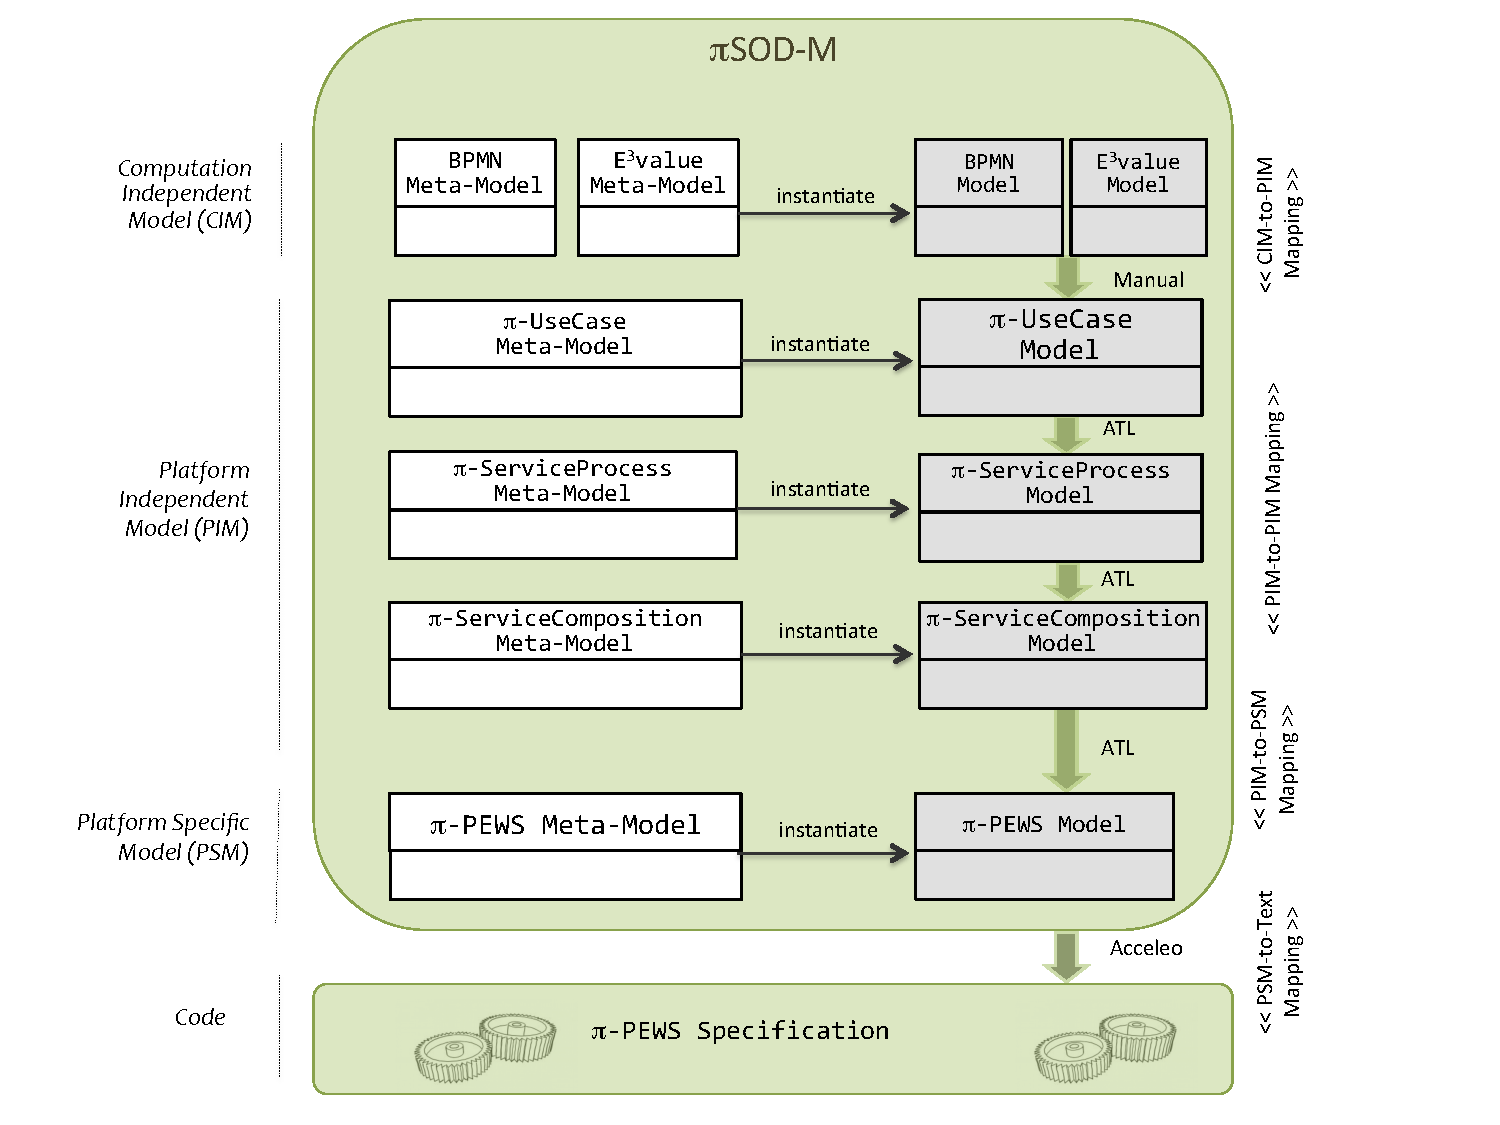
\includegraphics[width=0.75\textwidth]{./figures/piSOD-M_process.pdf}
\caption{\pisodm Overview.}
\label{fig:piSOD-M}
\end{figure}



%. . - -. . - -. . - -. . - -. . - -. . - -. . - -. . - -. . - -. . - -. . - -. . - -. . - -. . - -. . - -. . - -. . - -. . - -. . - -. . - -. . - -. . - -. . - -. . - -. . - -. . - -
\subsection{Computation Independent Models}
%. . - -. . - -. . - -. . - -. . - -. . - -. . - -. . - -. . - -. . - -. . - -. . - -. . - -. . - -. . - -. . - -. . - -. . - -. . - -. . - -. . - -. . - -. . - -. . - -. . - -. . - -

This level focuses on the highest-level view of the system, including its business and requirement specifications.
At this stage of the development, the structure and system processing details are still unknown or undetermined.
\pisodm uses the \textit{e$^3$value}~\cite{Gordijn02valuebased} and \textit{BPMN}~\cite{BPMN} meta-models for this purpose.

% .   .  .   .  .   .  .   .  .   .  .   .  .   .  .   .  .   .  .   .  .   .  .   .  .   .  .   .  .   .  .   .  .   .  .   .  .   .  .   .  .   .  .   .  .   .  .   .  .   .  .   .  .   .  .   .  .   .
\subsubsection{E$^3$value Meta-Model}
% .   .  .   .  .   .  .   .  .   .  .   .  .   .  .   .  .   .  .   .  .   .  .   .  .   .  .   .  .   .  .   .  .   .  .   .  .   .  .   .  .   .  .   .  .   .  .   .  .   .  .   .  .   .  .   .  .   .

The e$^3$value model  identifies the value/in\-for\-ma\-tion  exchange between system components (see Figure~\ref{fig:CIM:tpme3v}).
This model  represents a business case graphically as a set of value exchanges  ($\nabla$ $\triangle$) and value activities (rounded boxes) performed by business actors (squared boxes).
The model is well suited to enhance the understanding of the environment in which an application is being developed.
It defines \textit{dependency paths}, showing the value exchange between providers and end users when they ask for a service.
A dependency path has a direction and consists of a sequence of linked dependency nodes.
It starts with a \textit{start stimulus} node and ends with an \textit{end stimulus} node.
Dependency paths may also contain \textsl{OR} and \textsl{AND} elements (both for initiate and join alternative and parallel paths).

\begin{figure*}[h]
\center
\subfigure{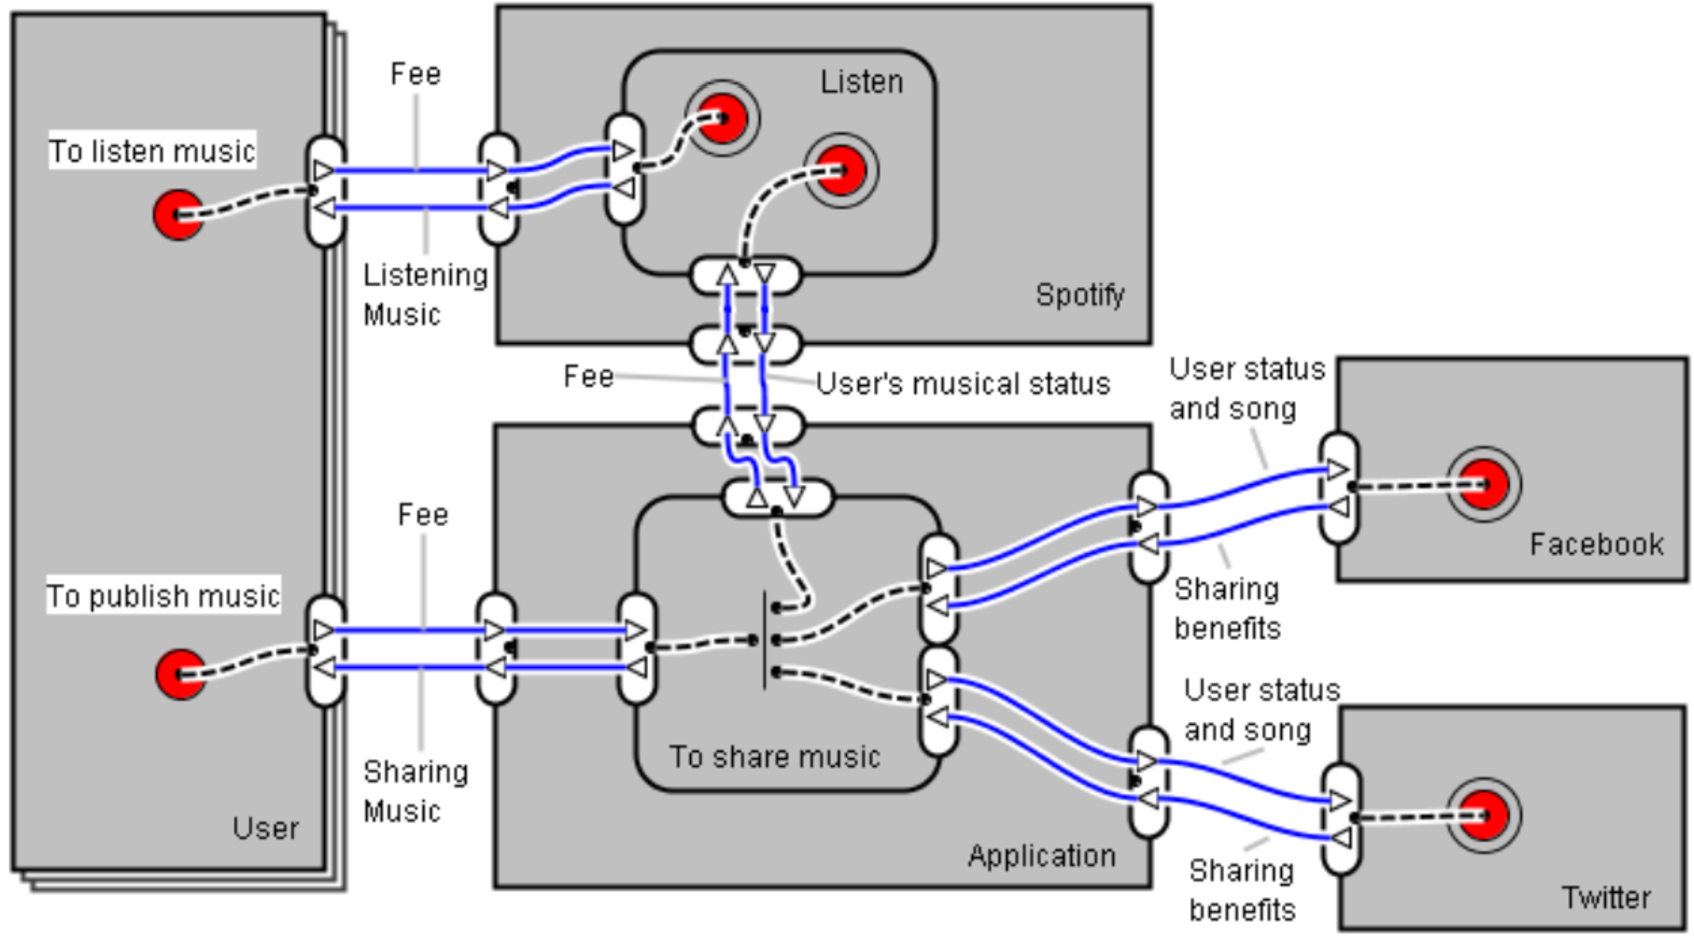
\includegraphics[width=0.55\textwidth]{./figures/e3value.pdf}}
~ 
\subfigure{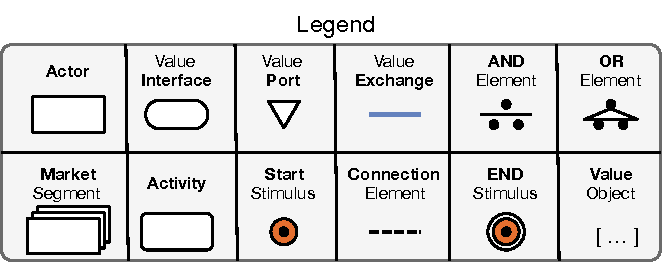
\includegraphics[width=0.4\textwidth]{./figures/3ValueKey.pdf}}
\caption{\label{fig:CIM:tpme3v} e3value model for ``To Publish Music''.}
\end{figure*}

\begin{example}[To Publish Music]\label{ex:toPublicMusic}
Let us consider the scenario ``To Publish Music'', used as a running example in this section:
An organization wants to provide the service based application ``To Publish Music'' that monitors the music listened by a user during some periods of time and sends the song title  to this person's Twitter and Facebook accounts.
In this way, the user will have her status synchronized in  Twitter and Facebook (i.e., either the same title is published in both accounts or it is not updated) with the title of the music she is listening in Spotify.
The application is based on three external actors ({\em Spotify, Twitter} and {\em Facebook}).
The following (external) services will be used by the application:

\begin{compactitem}
\item The  service   Spotify exports a meth\-od for obtaining information  about the music a given user is listening:
 {\sf\small get-Last-Song ( userid ): String}; 
\item The services Facebook and Twitter export meth\-ods for  updating the status of a given user:
 {\sf\small update-Status ( userid, new-status ): String};
\end{compactitem}




The e$^3$value model for ``To Publish Music'' is shown in Figure~\ref{fig:CIM:tpme3v}.
The e$^3$value value model shows Spotify and a private application (which is also a service) that directly interact with users for providing free services for listening and publishing information about music being listened by users. The private application interacts with Spotify for obtaining free information about the flow of music being listened by a user in return of a fee (i.e., premium subscription). Finally, the private application interacts with Facebook and Twitter for updating the user's status.
We can see this interaction as non material benefit sharing (as users subscribe to their networks and are active on them thanks to the private application).
\end{example}

The e$^3$value  model is used to model the (economic) value exchange among the actors involved in an application.
However, the e$^3$val\-ue model does not help to understand the business process of the application nor the conditions in which the different steps of this process are executed.
In order to face this shortcoming, our method proposes the BPMN meta-model as a tool for modelling this aspect of the application.



\subsubsection{BPMN Meta-Model}

BPMN~\cite{BPMN}  is a graphical representation that establishes the business process of the application through a high-level workflow.
The next example illustrates the use of this meta-model.

\begin{example}[To Publish Music \textit{(cont)}]\label{ex:toPublicMusicBPMN}
Figure \ref{fig:CIM:tpmbpmn} shows the BPMN model\footnote{Details on BPMN (Business Process Management Notation) can be found in http://www.bpmn.org/} of the scenario.
It starts by contacting the music service Spotify for retrieving the user's  musical status (activity {\sf Get Song}).
Twitter and Facebook services are then contacted in parallel for updating the user's status with the corresponding song title (activities {\sf Update Twitter} and {\sf Update Facebook}).
\end{example}
%
\begin{figure}[h]
\center
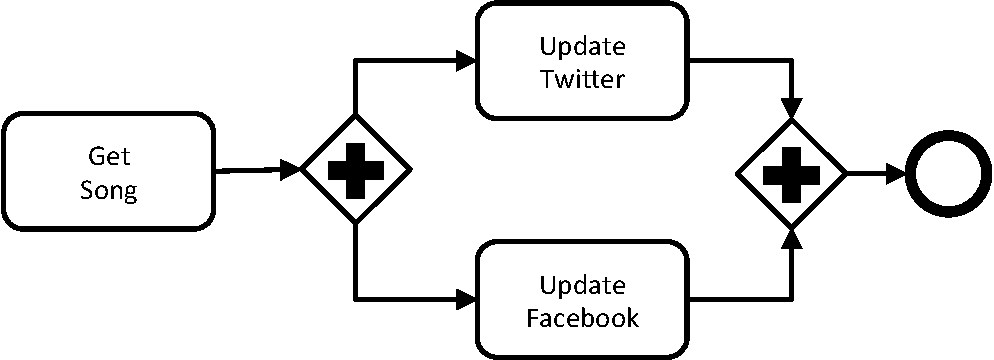
\includegraphics[width=0.4\textwidth]{./figures/SC.pdf}
\caption{\label{fig:CIM:tpmbpmn} BPMN model for ``To Publish Music''.}
\end{figure}

The CIM level models are the basis for the development of the application.
The information presented at this level is (manually) refined into PIM-level models of the method \pisodm described next.
Notice that, at this level, the models are (informally) used to describe both functional and non-functional requirements.

%. . - -. . - -. . - -. . - -. . - -. . - -. . - -. . - -. . - -. . - -. . - -. . - -. . - -. . - -. . - -. . - -. . - -. . - -. . - -. . - -. . - -. . - -. . - -. . - -. . - -. . - -
\subsection{Platform Independent Models}
%. . - -. . - -. . - -. . - -. . - -. . - -. . - -. . - -. . - -. . - -. . - -. . - -. . - -. . - -. . - -. . - -. . - -. . - -. . - -. . - -. . - -. . - -. . - -. . - -. . - -. . - -

This level focuses on the system functionality, hiding the details of any particular platform.
The specification defines those parts of the system that do not change from one platform to another.
Our method defines three PIM-level meta-models: \textit{$\pi$-UseCase}, \textit{$\pi$-Ser\-vice\-Pro\-cess} and \textit{$\pi$-ServiceComposition}.

 % .   .  .   .  .   .  .   .  .   .  .   .  .   .  .   .  .   .  .   .  .   .  .   .  .   .  .   .  .   .  .   .  .   .  .   .  .   .  .   .  .   .  .   .  .   .  .   .  .   .  .   .  .   .  .   .  .   .
\subsubsection{\textit{$\pi$-UseCase} Meta-Model}% .   .  .   .  .   .  .   .  .   .  .   .  .   .  .   .  .   .  .   .  .   .  .   .  .   .  .   .  .   .  .   .  .   .  .   .  .   .  .   .  .   .  .   .  .   .  .   .  .   .  .   .  .   .  .   .  .   .

Figure~\ref{fig:CIM:usecasemetamodel} shows the \textit{$\pi$-UseCase} meta-model.
This model is  to be the first representation of the application in terms of functionality, as well as to represent its non-func\-tion\-al requirements.
The notion of \textit{policy} is used to describe NFRs.
(Figure~\ref{fig:CIM:usecasemetamodel} highlights the concepts related to NFRs.)
The \textit{$\pi$-UseCase} meta-model extends the UML Use Case meta-model to describe NFRs with  the following  concepts:  {\sc Business service}, {\sc End consumer}, {\sc Requirement}, {\sc Use Case}, {\sc Composite Use Case}, {\sc Non-\-Func\-tion\-al Requirement}, {\sc Non-Functional} {\sc At\-tri\-bute} and {\sc Constraint}.
An {\sc End Consumer} is represented by an {\sc Actor}.
An  {\sc Actor} is related to {\sc Use Cases} (from the original UML definition), as a {\sc  Composite Use Case} is a set of actions performed by the system which can be broken into different {\sc Use Cases}.
{\sc  Business Service} aggregates several {\sc Use Cases},  a service can be expressed by one or more use cases.
 The {\sc Business Collaborator} concept is represented  by {\sc Packages}.
A {\sc Business Collaborator} denotes an external service or a system that interacts with the application that is being modeled.
Each {\sc Business Collaborator} combines the features described in each  {\sc Package}.
%Thus, the services functions can be specified as being grouped into packages.

 \begin{figure*}[h]
\center
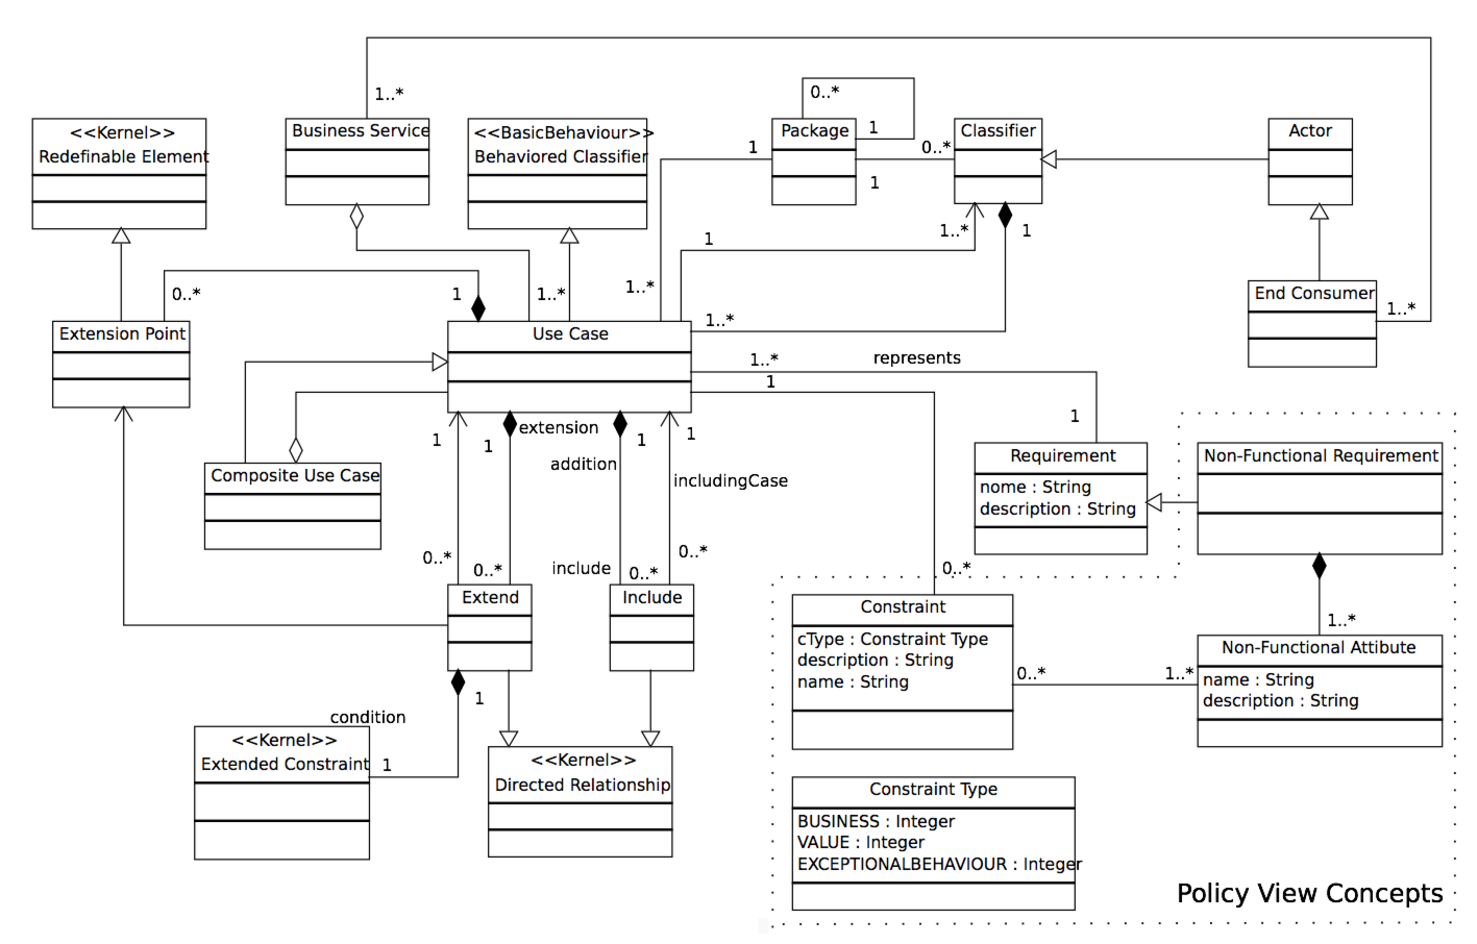
\includegraphics[width=0.8\textwidth]{./figures/UseCaseMetaModel.pdf}
\caption{\label{fig:CIM:usecasemetamodel} $\pi$-UseCase Meta-Model.}
\end{figure*}


 The {\sc Non-functional requirement} and {\sc Non-functional Attribute} concepts are represented by {\sc Use Cases} and {\sc Constraints}.
A {\sc Use Case} may have several {\sc Constraints}. Each {\sc Constraint} has a name, description, and a flag to indicate that it has to be  dynamically checked.
Each {\sc Con\-straint} is represented as a stereotyped ({\sf constraint}) use case.
There are three kinds of constraint:
\textit{(i)} A restriction may be associated to data ({\sc Value Constraint}), represented as the stereotype ``value'';
\textit{(ii)} A restriction may correspond to business rules (\textsc{Business Constraint}), represented as the stereotype {\sf ``business''}; and
\textit{(iii)} A restriction may describe {\sc Exceptional Behavior} constraints, represented as the stereotype {\sf ``exceptional\_behavior''}.
These constraints are shown in the next example.

\begin{example}[To Publish Music \textit{(cont)}]\label{ex:toPublicMusic2}
Figure~\ref{fig:CIM:piusecasetpm} shows a $\pi$-UseCase model for our example.
We consider that, besides the service composition for implementing the application, it is necessary to model  other requirements that represent the (i) conditions imposed by services usage --for example, the fact that both Facebook and Twitter require authentication protocol in order to call their methods for updating the wall; (ii) the conditions stemming from the business rules of the application logic, (e.g., the fact that the walls in Facebook and Twitter must show the same song title and if this is not possible then none of them is updated).

\begin{figure*}[h]
\center
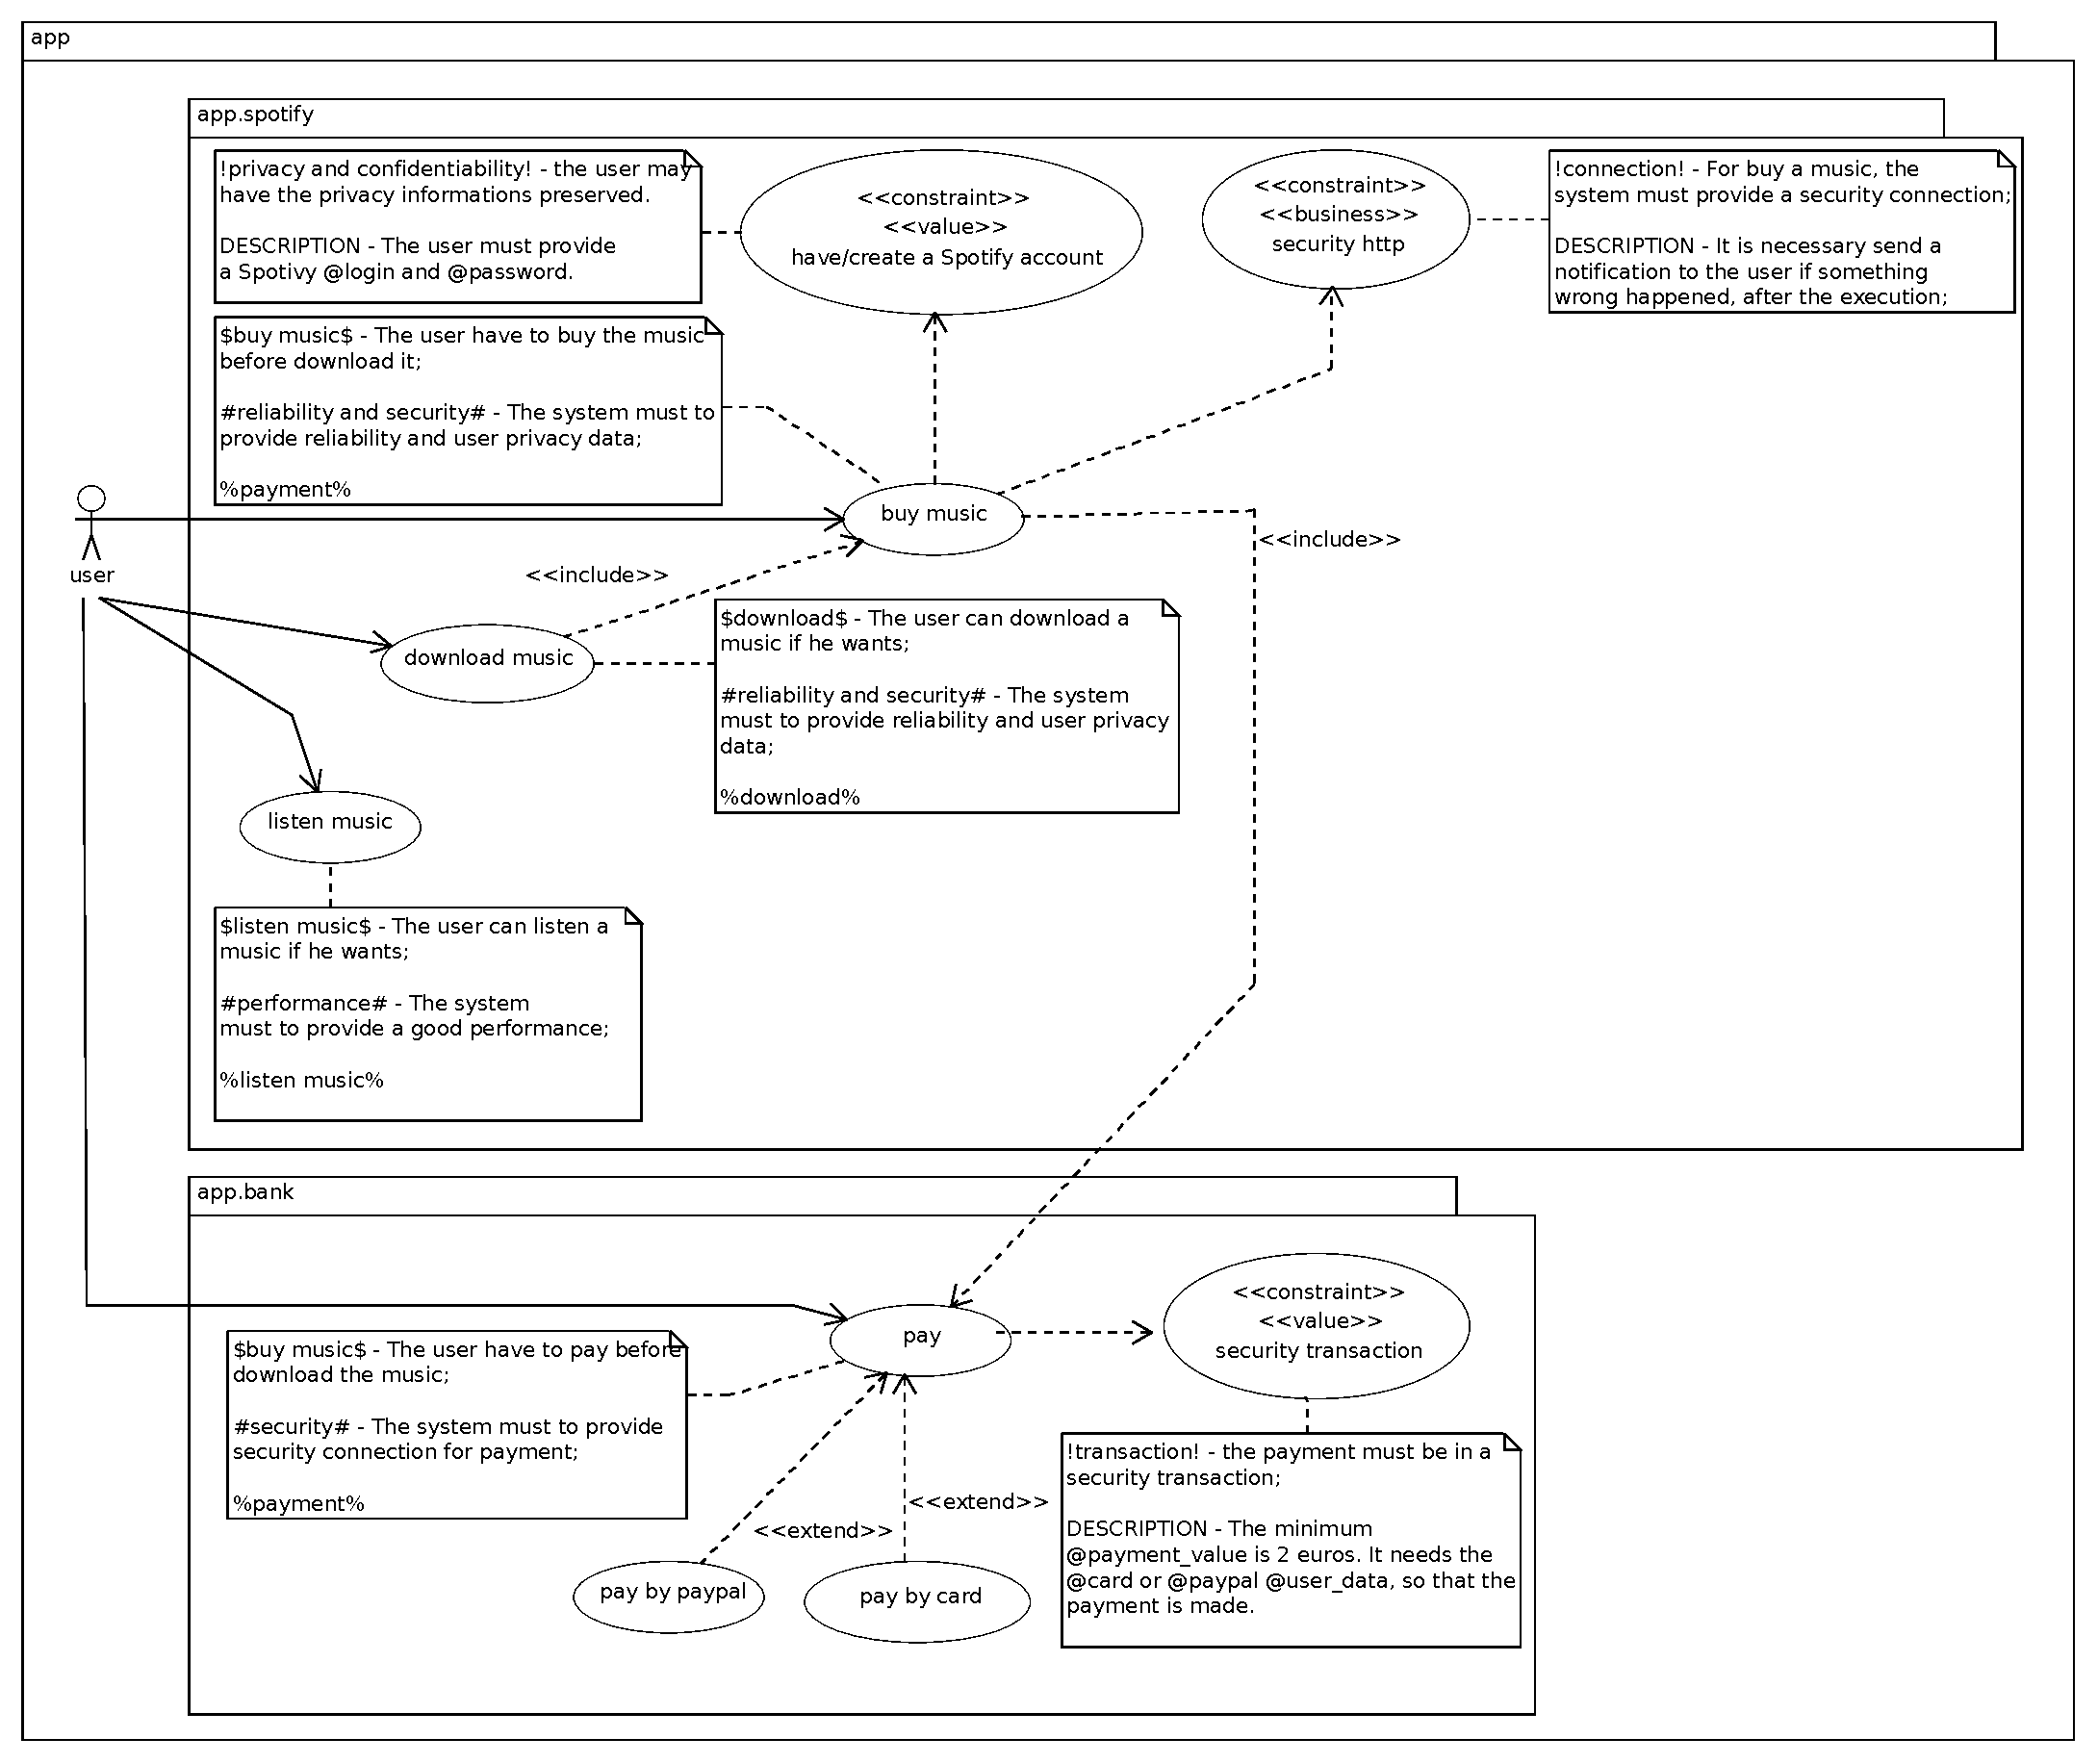
\includegraphics[width=0.8\textwidth]{./figures/UseCase.pdf}
\caption{\label{fig:CIM:piusecasetpm} $\pi$-UseCase model for ``To Publish Music''.}
\end{figure*}

The ``To Publish Music'' Business Service expects  the Facebook or Twitter user status to be changed every time a user starts listening a new song.
Therefore, it is necessary to perform a social network authentication with the users data. Each social network uses different services and different forms of authentication. The authentication constraint is required to update a music status. The restriction is stereotyped as a value constraint, because the users id and password are verified.  Figure \ref{fig:CIM:piusecasetpm} shows the buy music, download music, listen music and pay use cases. The process of buying a song requires the user private data for a Spotify account, and also a secure connection, represented as value and business constraint, respectively. For payment, the user must provide the data of payment card or PayPal account login and password, represented as value stereotype.
Minimum payment value is 2 euros.
%{\color{red} Talk about this model for the example.}
\end{example}

 % .   .  .   .  .   .  .   .  .   .  .   .  .   .  .   .  .   .  .   .  .   .  .   .  .   .  .   .  .   .  .   .  .   .  .   .  .   .  .   .  .   .  .   .  .   .  .   .  .   .  .   .  .   .  .   .  .   .
\subsubsection{\textit{$\pi$-ServiceProcess} Meta-Model}% .   .  .   .  .   .  .   .  .   .  .   .  .   .  .   .  .   .  .   .  .   .  .   .  .   .  .   .  .   .  .   .  .   .  .   .  .   .  .   .  .   .  .   .  .   .  .   .  .   .  .   .  .   .  .   .  .   .

The \textit{$\pi$-ServiceProcess} meta-model extends the UML activity diagram with the concept of \textit{contract} to represent constraints over data and actions. This concept is used to model
groups  of  constraints  in the \textit{$\pi$-UseCase}.
In Figure~\ref{fig:CIM:serviceprocessmetamodel}, the concepts of the \textit{$\pi$-Ser\-vice\-Process} meta-model are: {\sc Contract}, {\sc Assertion}, {\sc Exceptional behavior}, {\sc Activity}, {\sc Ser\-vice Acti\-vi\-ty}, {\sc Action} and {\sc Constraint}.
The dotted part of the figure defines those concepts related to the representation of NFRs.

\begin{figure*}[h]
\center
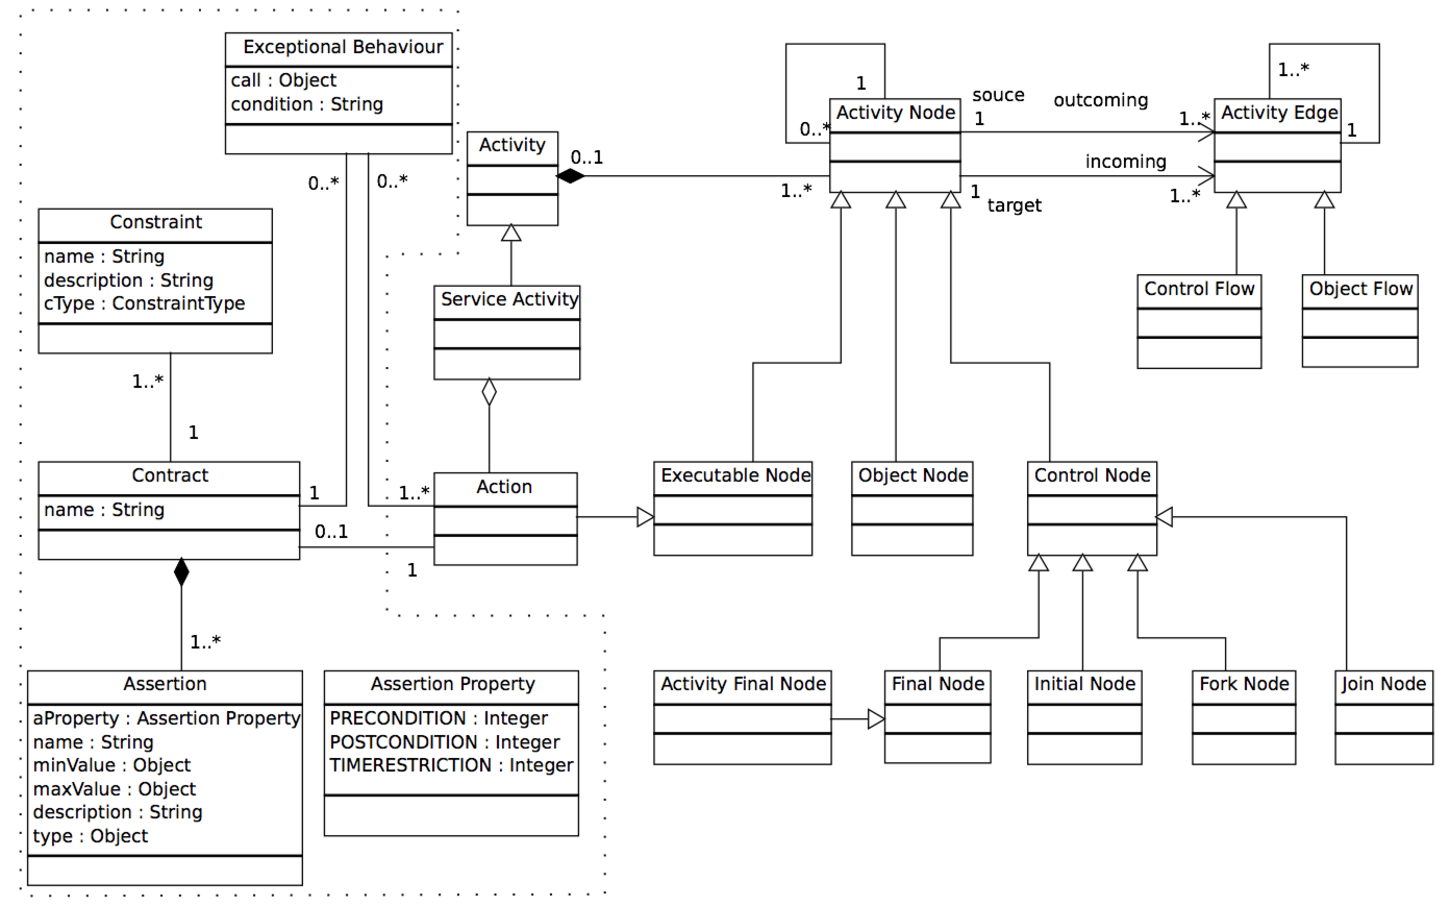
\includegraphics[width=0.8\textwidth]{./figures/ServiceProcessMetaModel.pdf}
\caption{\label{fig:CIM:serviceprocessmetamodel} $\pi$-Service Process Meta-Model.}
\end{figure*}

This model shows the set of logically related activities to be performed in a service-based application.
The activities of this model represent a behavior that is part of the business logic of the application.
A \textit{$\pi$-ServiceProcess}  model contains three main elements: (i) service process, (ii) service activity and (iii) activity contract. A service activity represents an operation that is part of the execution flow, and it is modeled as an {\sc Action}.
An activity contract represents the {\sc Non-functional Requirement}  that is also part of the execution flow of a service, identified  as a stereotyped activity ({\sf assertion}).
The {\sc Assertion}s associated to an {\sc Action} compose a {\sc Contract}. 
Using the concepts {\sc Contract} and {\sc Assertion} it is possible to specify each activity service, by defining its pre- and post-conditions.

\begin{example}[To Publish Music \textit{(cont)}]\label{ex:toPublicMusic3}
Considering the example scenario, the contract based process of activities  is shown in Figure \ref{fig:CIM:serviceprocess}. The buy music and publish music services (update Twitter and Facebook) have pre- and post-conditions assertions that are composed into a contract for each service. The buy music pre-conditions consist in verifying:
(i) if the User data are correct;
(ii) if the User is already logged in Spotify;
(iii) if bank account information are correct and;
(iv) if there are enough funds in the bank account to cover the payment.
A post-condition ensures the complete transaction and verifies if a notification was sent to the user and Spotify, about the payment authorization. There are four assertions for the buy music action, and each assertion has been detailed with the assertion property and predicate that must be verified. To update services, depending of each service, there may be different restrictions. As an example, a new verification of user data and message format is appropriate (maximum 140 characters), in the case of Twitter. In the case of Facebook, it is required that the user is already logged in Spotify and these data are the same as Facebook.
As post-condition, the application ensures that the Facebook service sends a notification of success.
To update Twitter a pre-condition is required, while to update Facebook it is necessary to check a pre-condition and a confirmation notice (modeled as post-condition).
As a pre-condition for ``twitter update'' it is necessary that (i) the music format is correct and (ii) the twitter login and password are correct for the update.
\end{example}

\begin{figure*}[h]
\center
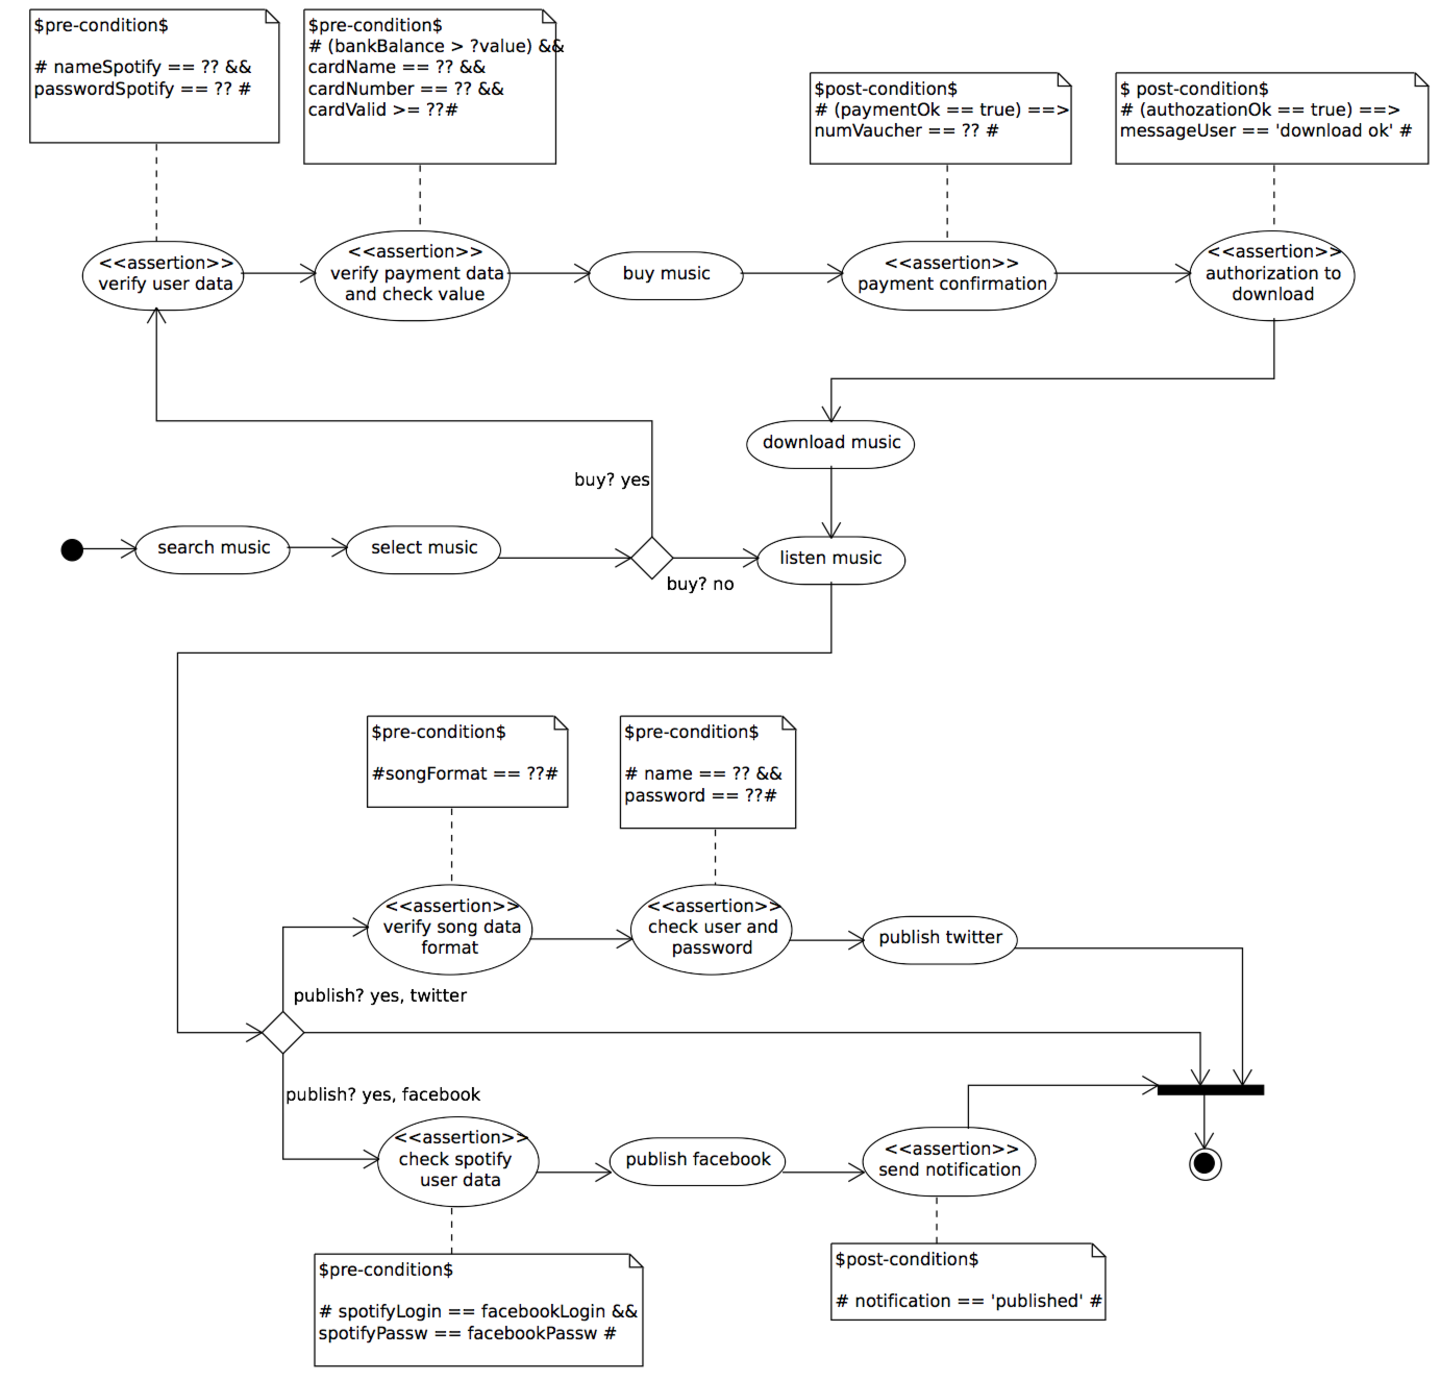
\includegraphics[width=0.8\textwidth]{./figures/ServiceProcess.pdf}
\caption{\label{fig:CIM:serviceprocess} $\pi$-ServiceProcess model for ``To Publish Music''.}
\end{figure*}

% .   .  .   .  .   .  .   .  .   .  .   .  .   .  .   .  .   .  .   .  .   .  .   .  .   .  .   .  .   .  .   .  .   .  .   .  .   .  .   .  .   .  .   .  .   .  .   .  .   .  .   .  .   .  .   .  .   .
\subsubsection{\textit{$\pi$-ServiceComposition} Meta-Model}% .   .  .   .  .   .  .   .  .   .  .   .  .   .  .   .  .   .  .   .  .   .  .   .  .   .  .   .  .   .  .   .  .   .  .   .  .   .  .   .  .   .  .   .  .   .  .   .  .   .  .   .  .   .  .   .  .   .

In Figure \ref{fig:e-scomposition-metamodel}, the $\pi$-Serv\-ice\-Com\-po\-si\-tion meta-model
provides meta-classes to represent workflows\footnote{Workflows are transformed into implemented service compositions.} that model  business processes.
The \textit{$\pi$-Serv\-ice\-Com\-po\-si\-tion} meta-model extends the UML activity  meta-model with the concept of  \textit{A-Policy}
to group contracts with similar non-functional requirements.
For instance, security and privacy restrictions may be grouped into a security policy.
 This meta-model defines:

\begin{compactitem}

\item A {\sc Business Collaborator} meta-class, to represent the classes of entities that collaborate in  business processes by performing some  action.
An instance of this meta-class is graphically a partition in the activity diagram.
A collaborator can be either internal or external to the system.
When the collaborator of the business is external to the system, the attribute {\sf IsExternal}\footnote{We use the {\sf sans serif} font for referring to classes defined using a meta-model.} of the collaborator is set to \textbf{true}.


\item {\sc Action}s, a kind of {\sc ExecutableNode}, are represented as a class activity instance of the meta-class \textsc{Action}.
A class action represents some type of transformation or processing.
There are two types of actions: i) a WebService (attribute Type is {\sf WS}); and ii) a simple operation called an {\sc ActivityOperation} (attribute Type is {\sc AOP}).

\begin{figure*}[h]
\centering
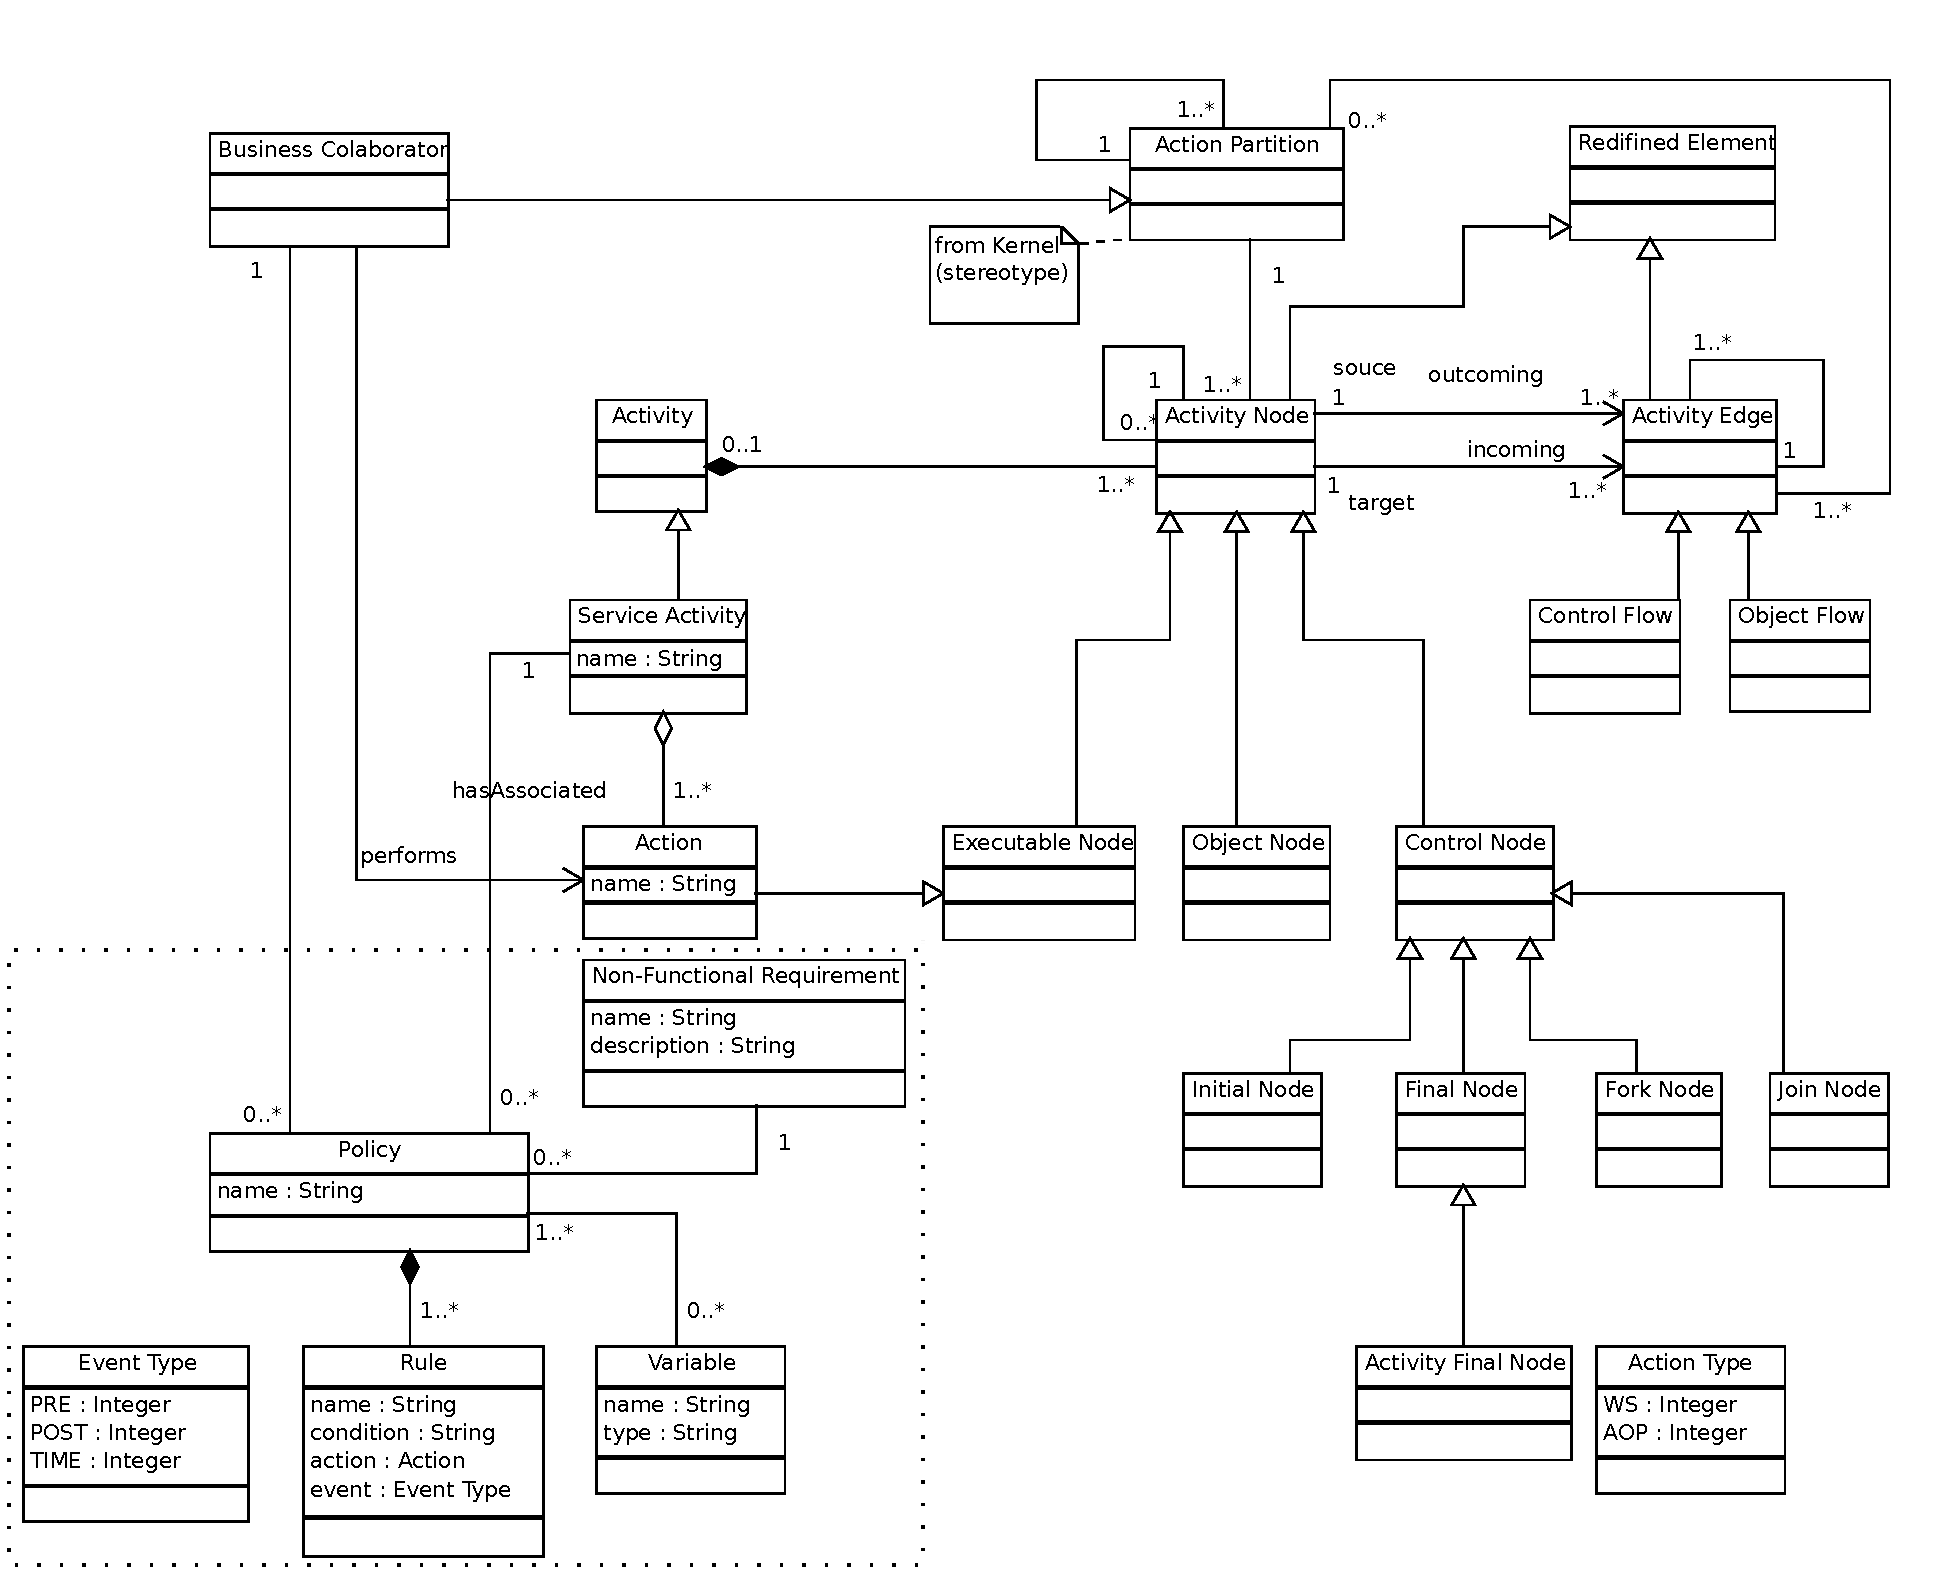
\includegraphics[width=0.8\textwidth]{./figures/PiServiceComposition}
\caption{$\pi$-Service Composition Meta-model.}
\label{fig:e-scomposition-metamodel}
\end{figure*}

\item The {\sc ServiceActivity} meta-class represents classes of composite activity types that must be carried out as part of a business service,  composed by  execu\-ta\-ble nodes.

\item In order to represent constraint types associated to services compositions, we defined the me\-ta- classes {\sc Rule} and {\sc A-policy} (see blue meta-classes in the $\pi$-Serv\-ice\-Com\-po\-si\-tion meta-model in Figure \ref{fig:e-scomposition-metamodel}).
We model non-func\-tion\-al constraints by using the notion of {\em A-policy}~\cite{Espinosa-Oviedo2011a,CIC:eovszmc09c}.
An {\em A-policy} is defined by attributes and rules.
The conditions of each rule are evaluated.
In case of failure, the actions of the rule will be performed.
The meta-class {\sc Rule} represents event-condition-action rules where the {\sc Event} part represents the moment in which a constraint  is evaluated.
An {\em A-policy} defines variables and operations that can be shared by the rules and that can be used for expressing their Event and Condition parts.

\end{compactitem}

\begin{figure*}[h]
\centering
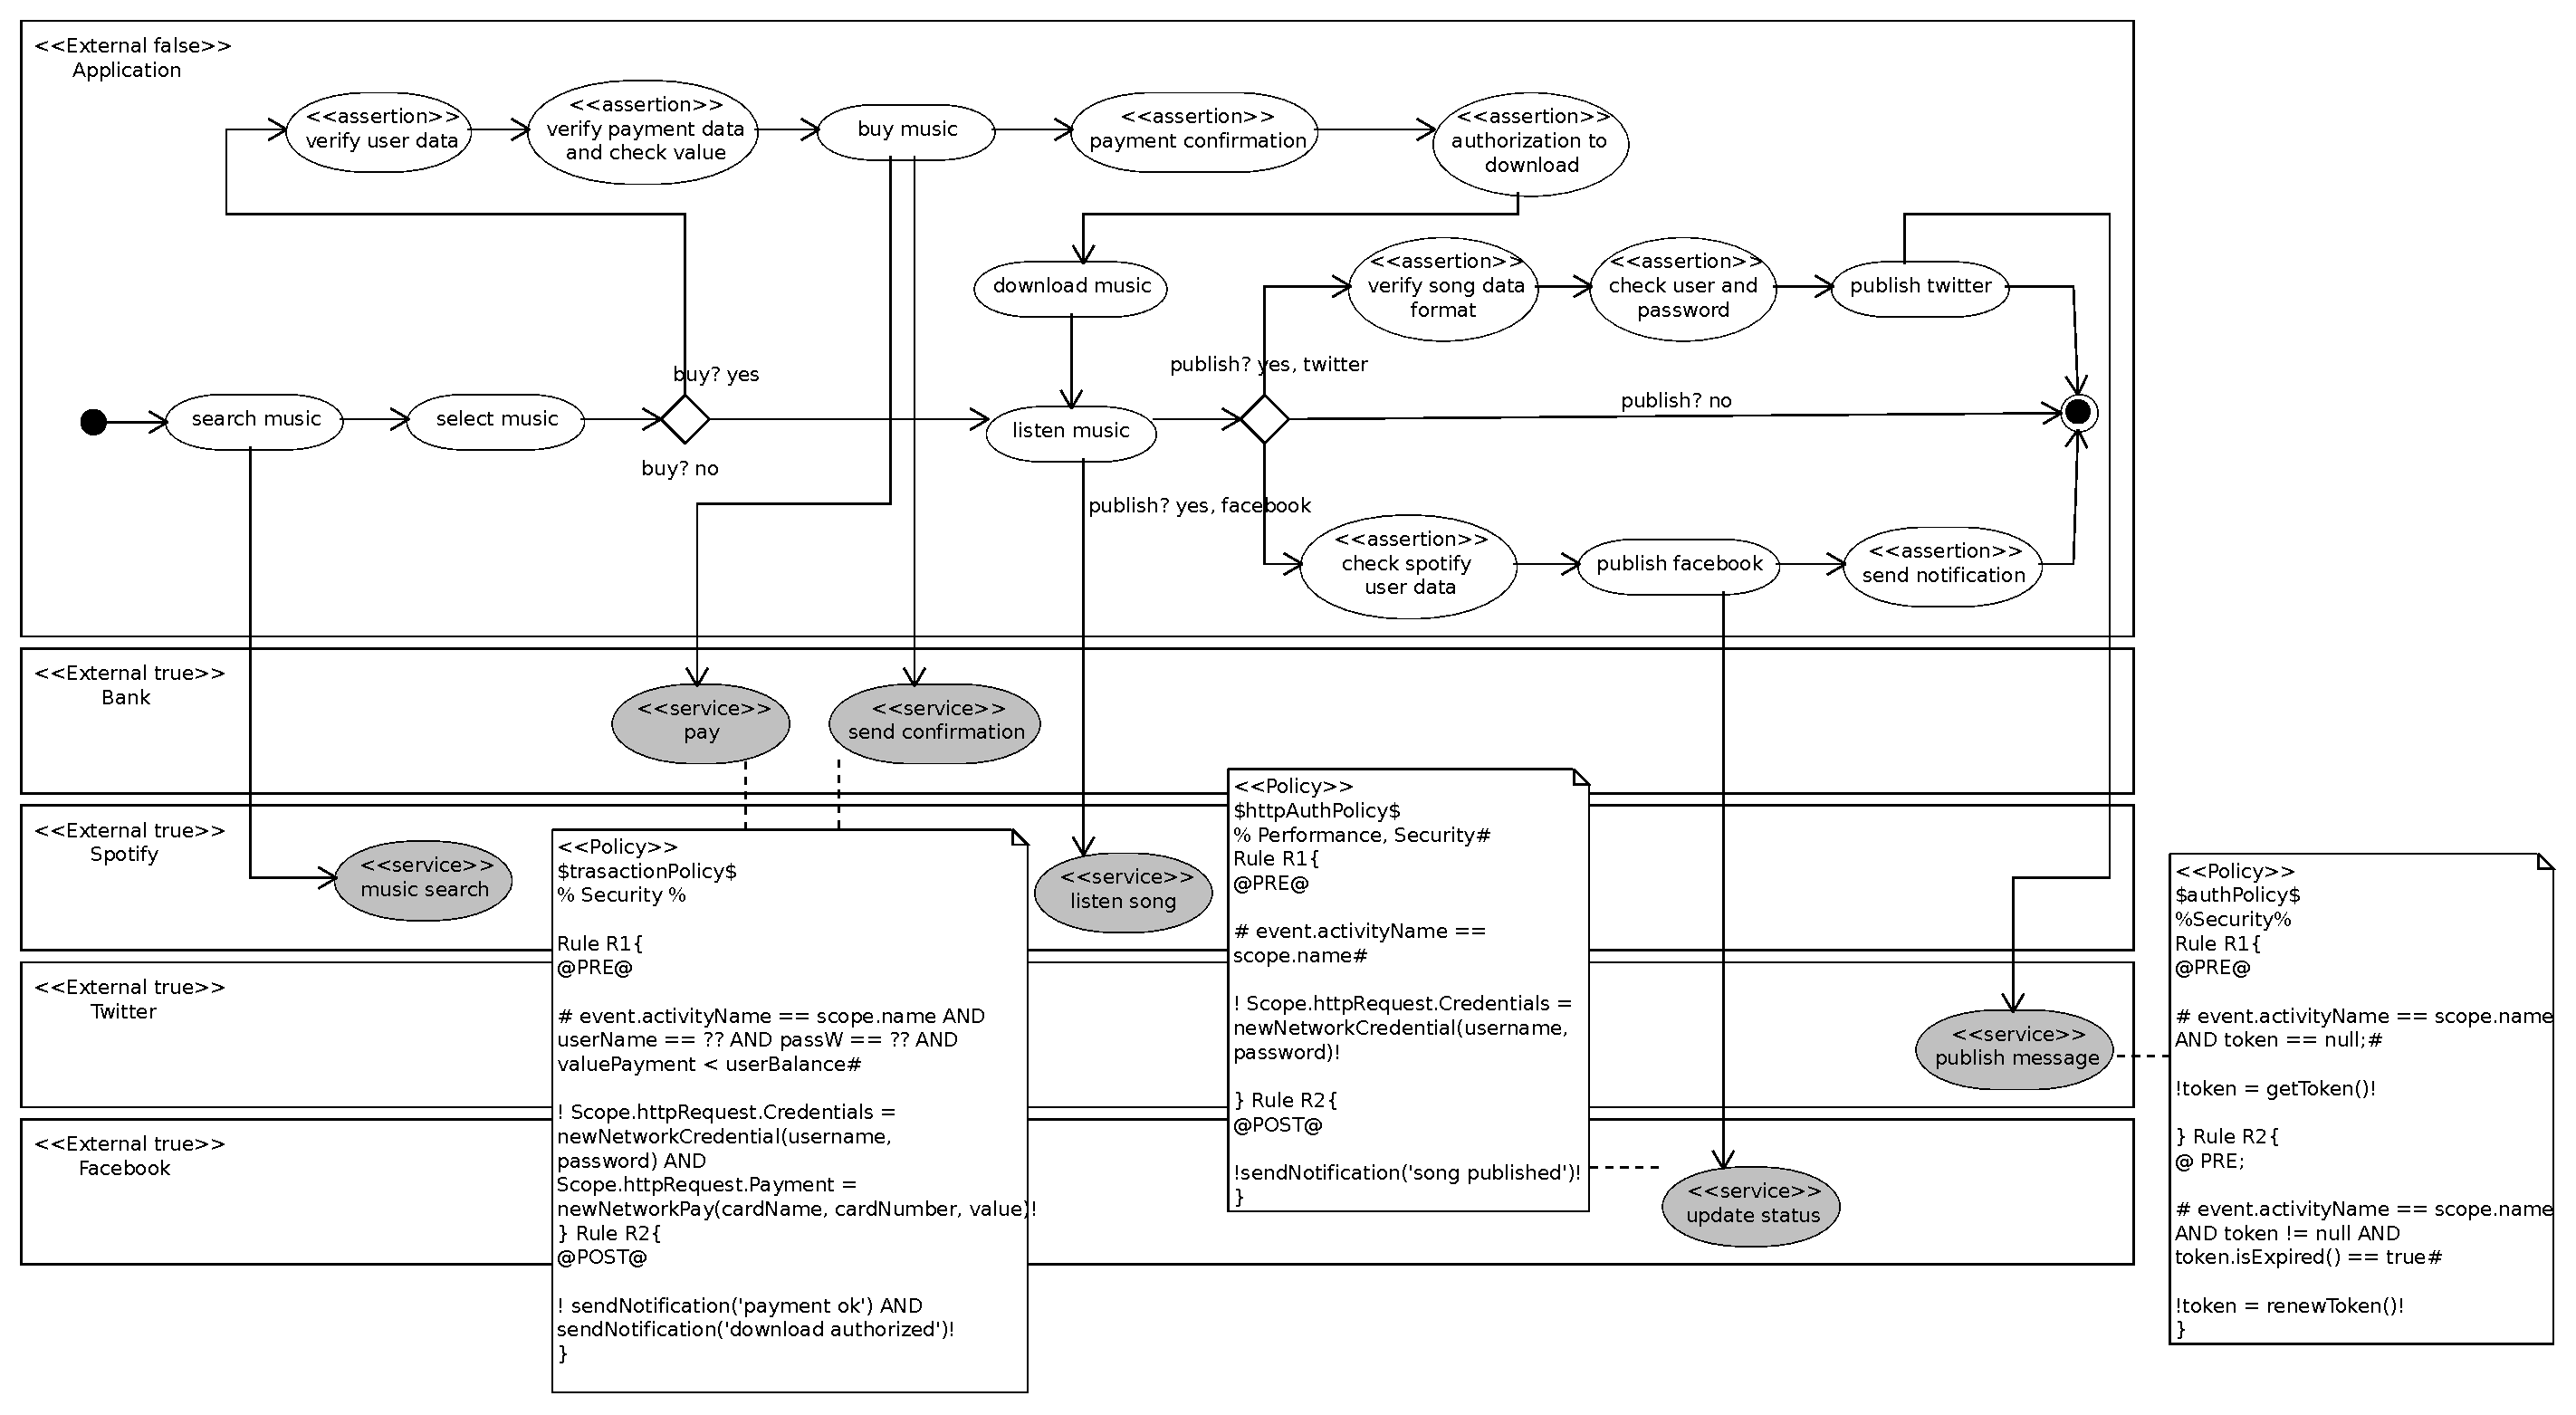
\includegraphics[width=0.95\textwidth]{./figures/piServiceComposition-toPublishMusic}
%{\color{red}\LARGE PLACIDO: Please change the names of the boxes in accordance to the explanation --Martin}
\caption{$\pi$-ServiceComposition Model for the ``To publish music'' business service.}
\label{fig:servicecompositionmodel}
\end{figure*}

\begin{example}[To Publish Music \textit{(cont)}]\label{ex:toPublicMusic4}
To illustrate the use of the $\pi$-Service Composition meta-model, we define a model for the ``To Publish Music'' scenario (Figure \ref{fig:servicecompositionmodel}).
 We model a business process with three service activities: {\em Listen Music}, {\em Publish Music} and {\em Confirmation}.
The {\em Publish Music} activity calls the {\em Facebook} and {\em Twitter} services.
Both {\em Facebook} and {\em Twitter} require authentication.
Two authentication policies are required, one for {\em Twitter} and another for {\em Facebook}.
%{\color{red} To be completed!.}
In this model, there are three external business collaborators ({\em Spotify, Twitter} and {\em Facebook}).
% \footnote{We use {\em italics} to refer to concrete values of the classes of a model that are derived from the classes of a meta-model.}).
The model also shows the business process of the application that consists of three service activities: {\em Listen Music}, {\em Publish Music} and {\em Confirmation}.
Note that  the activity {\em Publish Music} calls the actions of two service collaborators namely {\em Facebook} and {\em Twitter}.
Both {\em Facebook} and {\em Twitter} services require authentication protocols in order to execute methods that read and update the user data.
%A call to such services must be part of the authentication protocol required by these services.
In the example, we  associate two authentication policies, one for the open authentication protocol, represented by the class {\sf\small OAuthPolicy} at {\em Twitter}, associated to the activity  {\sf\small UpdateTwitter} (see Figure \ref{fig:servicecompositionmodel}).
In the same way, the {\em Facebook} class {\sf\small HTTPAuthPolicy}, for the http authentication protocol is associated to the activity {\sf\small UpdateFacebook}.
{\sf\small OAuthPolicy} implements the open authentication protocol.
The {\em A-policy} {\sf\small OAuthPolicy} has a variable {\sf\small Token}, used to store the authentication token provided by the service.
This variable is imported through the library {\sf\small OAuthPolicy.Token}.
The A-policy {\sf\small OAuthPolicy} defines two rules, both can be triggered by events of type {\sf\small ActivityPrepared}: (R$_1$): If no token has been associated to the variable {\sf\small token}, then a token is obtained ; and (R$_2$): if the token has expired, then it is renewed.
Notice that the code in the actions profits from the imported {\sf\small OAuthPolicy.Token} for transparently obtaining or renewing a token from a third party.
{\sf\small HTTPAuthPolicy} implements the HTTP-Auth protocol.
The A-policy imports an http protocol library and it has two variables {\sf\small username} and {\sf\small password}.
The event of type {\sf\small ActivityPrepared} is the triggering event of the rule {\sf\small R$_1$}.
On the notification of an event of that type, a credential is obtained using the username and password.
\end{example}

Once the $\pi$-Service Composition Model is defined,  it can be transformed into a lower level model (in our case, $\pi$-PEWS) to support code generation as described in the next section.


%. . - -. . - -. . - -. . - -. . - -. . - -. . - -. . - -. . - -. . - -. . - -. . - -. . - -. . - -. . - -. . - -. . - -. . - -. . - -. . - -. . - -. . - -. . - -. . - -. . - -. . - -
\subsection{Platform Specific Models}
%. . - -. . - -. . - -. . - -. . - -. . - -. . - -. . - -. . - -. . - -. . - -. . - -. . - -. . - -. . - -. . - -. . - -. . - -. . - -. . - -. . - -. . - -. . - -. . - -. . - -. . - -

This level focuses on the functionality, in the context of a particular implementation platform.
Models at this level put together the platform-independent view with the specific aspects of the platform to implement the system.
These models  can be automatically translated into actual computer programs.
We have defined one meta-model at this level.

\textit{$\pi$-PEWS} provides con\-cepts for modelling service compositions.
Instances of this meta-model are textual descriptions of service compositions that can be translated into any service composition language, such as BPEL~\cite{bpel03} or PEWS~\cite{BaCAM05,Placido2010LTPD}.
%
PEWS~\cite{BHM06,Placido2010LTPD} is a notation to express service compositions.
The language is based on the notion of Path Expressions~\cite{And79} and can easily be translated into any actual composition language, such as BPEL~\cite{bpel03}.
Figure~\ref{fig:PPEWSmetamodel} presents the $\pi$-{\sc Pews} meta-model, where we identify classes to describe:

\begin{compactitem}
\item Service compositions: {\sc Namespace} represents the interface exported by a service, {\sc Operation} represents a call to a service method, {\sc CompositeOperation}, {\sc Operator} and {\sc Path}  denote service compositions.
A {\sc Path} can be an {\sc Operation} or a {\sc Compound Operation}.
A {\sc Compound Operation} is defined using an {\sc Operator}.
The language defines operators to denote guarded operations ($[C]S$); sequential ($\ . \ $), parallel ($\ \| \ $) and alternative ($\ + \ $) compositions; as well as sequential ($*$) repetition.
\item {\em A-Policies} that can be associated to service compositions:  {\sc A-Policy}, {\sc Rule}, {\sc Event}, {\sc Condition}, {\sc Action}, {\sc State}, and {\sc Scope}.
\end{compactitem}

Figure~\ref{fig:PPEWSmetamodel} shows that each {\sc A-Policy} is associated to a {\sc Scope} that can be either an {\sc Operation} (e.g., an authentication protocol associated to a method exported by a service),  an {\sc Operator} (e.g., a temporal constraint associated to a sequence of operators) or a {\sc Path}.
Each {\sc A-Policy} groups a set of ECA rules with a classic semantics, i.e, {\em when an event of type E occurs, if condition C is verified then execute the action A}.
In this way, an {\em A-policy} represents a set of reactions to be possibly executed when one or several events are notified.

\begin{figure*}[h]
\centering
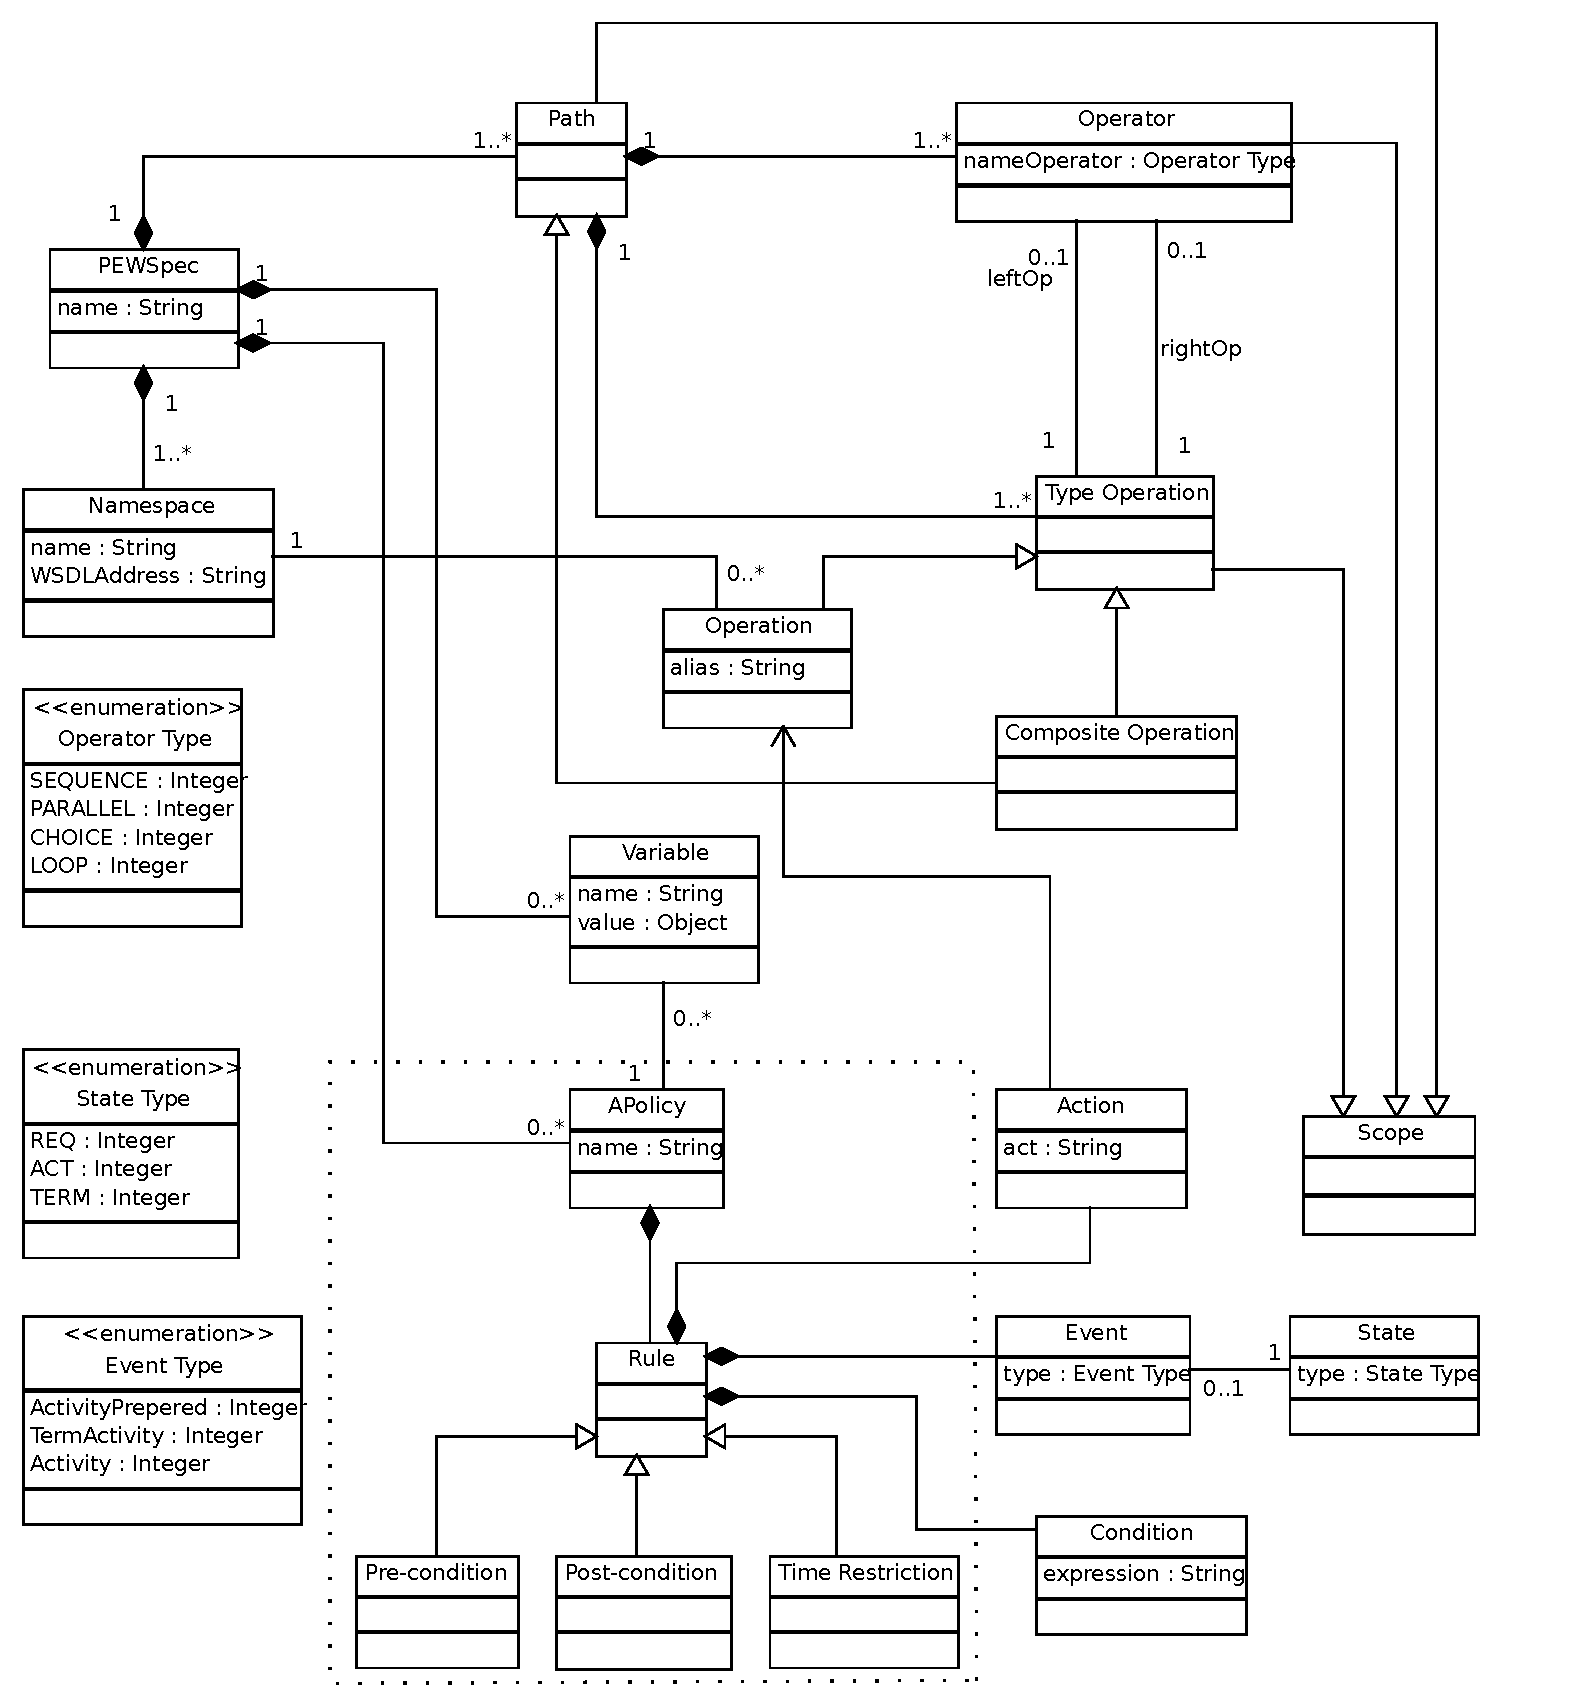
\includegraphics[width=0.7\textwidth]{./figures/PEWSMetamodel}
\caption{$\pi$-{\sc Pews} Meta-model.}
\label{fig:PPEWSmetamodel}
\end{figure*}

\begin{example}[To Publish Music \textit{(cont)}]\label{ex:toPublicMusic5}
Figure \ref{fig:Specific-Contract-Representation} shows the $\pi$-PEWS code resulting from the $\pi$-service composition model of our example.
The code contains namespaces and definitions (obtained from the business collaborators of the $\pi$-SCM model), a workflow expression \textit{(Path)} containing operation calls and contracts (derived from the \textit{A-Policies}).
\end{example}

\begin{figure*}[h]
\centering

\includegraphics[width=0.5\textwidth]{./figures/pi-pewsSpecification-toPublishMusic}
\caption{$\pi$-PEWS Specific and Policy Representation.}
\label{fig:Specific-Contract-Representation}
\end{figure*}


\section{Transformation Rules}\label{sec:mmrules}


%..--..--..--..--..--..--..--..--..--..--..--..--..--..--..--..--..--..--..--..--..--..--..--..--..--..--..--..--..--..--..--..
%\subsubsection{$\pi$-{\sc Pews}  meta-model}\label{sec:pewsmetamodel}
%..--..--..--..--..--..--..--..--..--..--..--..--..--..--..--..--..--..--..--..--..--..--..--..--..--..--..--..--..--..--..--..

\pisodm  proposes intra-level transformation rules between $\pi$-use case to $\pi$-service process models, $\pi$-service process to $\pi$-service composition  models, as well as inter-level transformation rules between $\pi$-service composition to $\pi$-PEWS models. 
These rules are used to build a semi-automatic tool (the \pisodm  plugin for Eclipse).
The transformations from CIM to PIM level models are not automatized, due to the informal nature of CIM level.
 
% _ . _ . _ . _ . _ . _ . _ . _ . _ . _ . _ . _ . _ . _ . _ . _ . _ . _ .
\subsection{From $\pi$-UseCase to the $\pi$-ServiceProcess}
% _ . _ . _ . _ . _ . _ . _ . _ . _ . _ . _ . _ . _ . _ . _ . _ . _ . _ .

The refinement of a (composite) $\pi$-Use Case model into a $\pi$-Service Process model is driven by the principle of expressing a set of $\pi$-use cases (i.e., use cases with constraints)   in terms of  a business process.
The resulting model consists of actions related by a control flow and contracts specifying NFPs. 

As defined by the $\pi$-ServiceProcess  meta-model (Figure~\ref{fig:CIM:serviceprocessmetamodel}) an {\sc Activity Service} consists of a composition of  entities of type {\sc Action}. 
Thus, every {\sf $\pi$-use case} is transformed into an {\sf Action} of the target $\pi$-Service Process model.  
Every {\sf Extend} relationship identified in a $\pi$-Use Case model is
transformed into a  {\sf Fork node}~\cite{valeriaThesis,placidoPhDThesis2012}.
If the {\sf Extend} relationship concerns just one {\sf use case}, it is transformed into an {\sf Action} inside one flow of the fork node. 
Otherwise, several  {\sf use cases} are transformed into different {\sf Actions} that belong to different flows departing from the fork node.   
%
A {\sf Constraint} associated to a {\sf Use Case}  is transformed into an  {\sf Assertion}.  
The set of resulting assertions  are grouped into a {\sf Contract}.
Constraints are transformed according to their type:
{\sc Business} constraints and {\sc Value} constraints with the {\sf  isExceptionalBehaviour} at\-tri\-bute set to false are transformed into {\sf Assertion}s;
{\sc Value } constraints with the {\sf  isExceptionalBehaviour} attribute set to true are transformed into {\sf Exceptional behavior}s.

In order to transform constraints of type {\sf Value Constraint}, the designer specifies thresholds to be associated to the assertions of a contract.
By default, value constraints are transformed into pre-conditions and business constraints are transformed into post-conditions. 
  
The relationships of type  {\sc Extend} and {\sc Include}  determine the way the business process is expressed as a workflow.  
The generated workflow is composed by {\sf Fork} and {\sf Join} nodes,  {\sc Control flow} constructors, as well as entities of type {\sc Action}.

{\sf Include} use case entities are transformed into an {\sf Action} sequence.
A {\sc Use case} element is transformed into an {\sf Action}. 
A set of $n$ {\sc Use cases} is transformed into an  $n-1$ {\sf Object flow} elements. 
%
Details of these transformations can be found in~\cite{SouzaNeto:2012}.

\begin{example}[To Publish Music \textit{(cont)}]\label{ex:toPublicMusicT1} 
The transformation rules have been applied to the model in Figure~\ref{fig:CIM:piusecasetpm} to obtain the $\pi$-Service Process model for our example (Figure~\ref{fig:CIM:serviceprocess}).



The ``listen music'' use case is transformed into a Service Action that  represents a Spotify  function to be invoked to play music. 
For the ``publish music'' use case,  constraints are transformed into a set of assertions that are grouped into a Contract ({\sf ``publishMusicContract''}) associated to the Action {\sf ``publishMusic''}. 
The use case ``download music''  includes the payment process to buy the music. 
Thus, these use cases  are transformed into {\sf Actions}, and a {\sf Service Activity} that aggregates these {\sf Actions}.   
This \textsf{Service Activity} is transformed into a sequence flow on the $\pi$-service process model.
The same rule is applied to the ``publish music'' use case, which has two extended use cases, to publish on Twitter and Facebook.
 \end{example}

% _ . _ . _ . _ . _ . _ . _ . _ . _ . _ . _ . _ . _ . _ . _ . _ . _ . _ .
\subsection{From $\pi$-ServiceProcess to $\pi$-ServiceComposition}
% _ . _ . _ . _ . _ . _ . _ . _ . _ . _ . _ . _ . _ . _ . _ . _ . _ . _ .

The transformation  of a  $\pi$-Service Process model into a $\pi$-Service Composition model groups {\sf Contracts} into {\sf A-Policies} and {\sf Actions} into {\sf Service Activities}.   
Each {\sf Assertion} of a {\sf Contract} is transformed into a {\sf Rule}. 
{\sf Rules}  concerning the same NFP  are grouped into {\sf A-Policies}. 
Each {\sf Assertion} of a {\sf Contract} is transformed into a {\sf Rule:Condition} attribute. 
If the {\sf Assertion} has a value type, the name and the attributes are transformed into {\sf Variables} in the target model.  
The {\sf Assertion: aProperty} attribute can have different transformations, according to: 
\textit{(i)} a {\sf Precondition} is transformed into {\sf Pre};
\textit{(ii)} a {\sf Post-Condition} is transformed into a {\sf  Post};
\textit{(iii)} a {\sf TimeRestriction} is transformed into {\sf Time}.

Some elements of the $\pi$-service composition model are obtained from the $\pi$-UseCase model: 
A {\sf Package} in the $\pi$-use case model is transformed into a {\sf Business Collaborator};
\textsf{Non-Functional Attributes} of the $\pi$-use case model are grouped into \textsf{Non-Functional requirements} of the $\pi$-ServiceComposition model. 
These requirements are associated to a \textsf{Policy} (from the $\pi$-ServiceProcess model).




{\sf Actions} and {\sf Service activity} of a $\pi$-Service Process model are transformed into their hom\-onym concepts of the $\pi$-Service Composition model.
Finally, {\sf Actions} are grouped into  a {\sf Business collaborator}.


\begin{example}[To Publish Music \textit{(cont)}]\label{ex:toPublicMusicT5}
Considering the example scenario, the model in Figure~\ref{fig:servicecompositionmodel} was obtained by applying the rules above to the model depicted by Figure~\ref{fig:CIM:serviceprocess}.  
The ``securityLoginPolicy'' consists of a set of {\sf Rules} that were transformed from the {\sf Assertions} in $\pi$-service process model. 
The information about Facebook and Spotify (both of them {\sf Business Collaborators}) come from entity of type {\sc Package} in the $\pi$-use case
model.
\end{example}

% _ . _ . _ . _ . _ . _ . _ . _ . _ . _ . _ . _ . _ . _ . _ . _ . _ . _ .
\subsection{From $\pi$-ServiceComposition to $\pi$-PEWS}
% _ . _ . _ . _ . _ . _ . _ . _ . _ . _ . _ . _ . _ . _ . _ . _ . _ . _ .

This section describes the PIM to PSM transformations from a $\pi$-Service composition mod\-el to a $\pi$-PEWS model. 
We distinguish two groups of rules: \textit{(i)} those transforming service composition entities into workflows; and \textit{(ii)} those transforming  A-Policies into Contracts.

Single actions ({\sf Action} and {\sf
Action:name}) are transformed into individual service {\sf Operations}.
Complex actions (rep\-re\-sented by {\sf ServiceActivity}  and  {\sf
ServiceActivity:name}) are transformed into (named) composite
operations that defines a (named) workflow of the application.
Composition patterns expressed using  {\em merge, decision, fork} and {\em join} are transformed into their corresponding workflows of the $\pi$-PEWS model.

A-Policies defined for the entities of a $\pi$-service composition model generate {\sf A-policy} entities, named according to the names expres\-sed in the source model.
The transformation of the rules expres\-sed in a $\pi$-service composition is guided by the event types associated to these rules. 
The variables associated to an A-Policy expressed in a $\pi$-service composition model as {\sf $<$Variable:name, Variable:type$>$} are transformed into  {\sf Variable}, with  {\sf Name} and {\sf Type} attributes specified from the elements {\sf Variable: name} and {\sf Variable:type} of a $\pi$-service composition model.
%
Events of type {\sf Pre}, {\sf Post} and {\sf Time} generate, respectively, {\sf Pre-conditions}, {\sf Post-condition} and {\sf TimeRestrictions}.

\begin{example}[To Publish Music \textit{(cont)}]\label{ex:toPublicMusicT6}
Figure \ref{fig:Specific-Contract-Representation} shows the $\pi$-PEWS code resulting from the $\pi$- service composition model (Figure~\ref{fig:servicecompositionmodel}) of our scenario example.
\end{example}


\subsection{Implementation}
We have developed tools for aiding the user to define and transform the models for all the levels, except for the CIM into PIM level, which should be manually performed.
Our tool is implemented as a series of Eclipse plug-ins: 
\begin{compactitem}
\item 	We  used the Eclipse Modeling Framework (EMF)\footnote{The EMF project is a modeling framework and code generation facility for building tools and other applications based on a structured data model.}   to implement the  $\pi$-Service Composition and $\pi$-{\sc Pews}  meta-models. 
From these meta-models, we  developed plug-ins to support their graphical representation.

\item	 We used  ATL\footnote{http://eclipse.org/atl/. An ATL program is basically a set of rules that define how source model elements are matched and navigated to create and initialize the elements of the target models.}
for implementing the  mappings between models.

\item 	We  used Acceleo\footnote{http://www.acceleo.org/pages/home/en} to implement  the code generation plug-in to generate executable code. 
It takes a $\pi$-PEWS model and generates the code to be executed by the {\em
A-Policy} based service composition execution environment.
\end{compactitem}


\section{Applying \pisodm: The \FlyingPig\ Case Study}
\label{sec:flyingPig}


To validate the applicability of our method we have developed a case study concerning risk assessment for financial companies as implemented by the ORCA System\footnote{The ORCA System is a trademark of GCP Global (www.gcpglobal.com).}.
Risk assessment is implemented by an interactive business process based on the exchange of questionnaires used to evaluate the risks implied by the client business practice.
Examples of business practices are: the conditions and protocols used to perform confidential transactions, the physical security to access reserved areas (such as computing server installations).
The information gathered by the questionnaires is used to evaluate whether there are risky practices within the business processes, as well as to propose amendments to these practices.
The ultimate goal of the risk assessment is to determine a degree of compliance to existing standards.
By analyzing the questionnaires, ORCA detects risky practices, proposes solutions and triggers further assessment processes to ensure that the solutions have been implemented.

Our goal is to model a service based application (\FlyingPig), for providing risk assessment as a service.
In order to provide this functionality, \FlyingPig\ benefits from ORCA's legacy services providing storage, assessment and data visualization functions.
%
In the next sections we apply \pisodm to develop the \FlyingPig\ risk assessment system.
The models presented were generated as a result of interacting with software developers at GCP Global.



%. . - -. . - -. . - -. . - -. . - -. . - -. . - -. . - -. . - -. . - -. . - -. . - -. . - -. . - -.fig:E3valuemodel . - -. . - -. . - -. . - -. . - -. . - -. . - -. . - -. . - -. . - -. . - -. . - -
\subsection{Computation-Independent Models (CIM)}
%. . - -. . - -. . - -. . - -. . - -. . - -. . - -. . - -. . - -. . - -. . - -. . - -. . - -. . - -. . - -. . - -. . - -. . - -. . - -. . - -. . - -. . - -. . - -. . - -. . - -. . - -

Figure~\ref{fig:E3valuemodel} shows the value model for the \FlyingPig\ application.
It is a business model that graphically represents a business case as a set of value exchanges ($\triangleright$ and $\triangleleft$) and value activities (rounded boxes) performed by business actors (squared boxes).
We identify two business actors: \textsl{ORCA} and \textsl{Broker}.
Brokers emit requests for risk assessment for one or more companies.
ORCA has two value activities which are services that provide an economical benefit:  \textsl{Identify Amendments} and \textsl{Assess Risk Situation}.
The values exchanged between ORCA and the brokers are:
(i) \textsl{Questionnaire and Evidences} filled with information about the client company;
(ii) \textsl{Amendments} which are ORCA's rec\-om\-men\-da\-tions, based on the data provided by the answers to questionnaires;
(iii) \textsl{Evaluation Reports} for the client companies;
and
(iv) the risk assessment \textsl{fee}.
%
The dependency path in Figure~\ref{fig:E3valuemodel} initiates with the need of assessment emitted by a particular company.
Once this need has been declared, the value exchanges between ORCA and Broker are triggered.
The client company provides ORCA with information (answers to a questionnaire), evidence (to support the information) and a fee (monetary value).
In the next step, ORCA suggests amendments (recommendations to change practices) and provides an evaluation report.

\begin{figure*}[h]
\centering
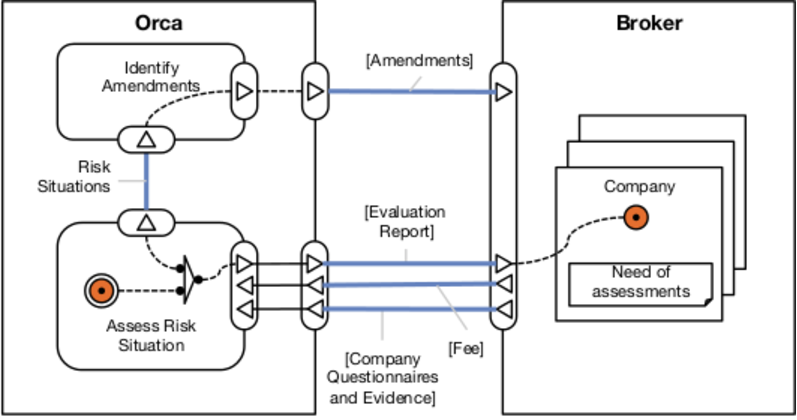
\includegraphics[width=0.45\textwidth]{./figures/3ValueModel.pdf}
%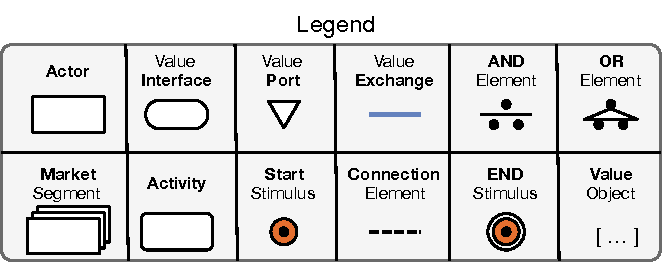
\includegraphics[width=0.4\textwidth]{./figures/3ValueKey.pdf}
\caption{E3value model for \FlyingPig.\label{fig:E3valuemodel}}
\end{figure*}

Figure~\ref{fig:BPMNmodel} shows the BPMN model
for the \FlyingPig\ scenario. This model is partitioned for better understanding the value exchanging process.
The model includes two pools representing the \textsl{ORCA} system and the \textsl{Brokers}.
Brokers have two lanes, the client \textsl{Company} and a \textsl{User}.
The user is a contact member of the company, who  coordinates the assessment process.
This process  involves other members of the company as well.
%
The risk assessment process starts after a request from a company.
This corresponds to the value model, in which the start stimulus triggers the whole process.
The request leads to the definition of a group of users that will answer questionnaires to evaluate risk.
Other tasks include amending a ``risky situation'' as well as producing evidence to show that a specific risk has been eliminated\footnote{Risky situations include  material facts such as not facilitating access to physically disabled people in a bank agency or having an unsecured access to the premises of the company.
They can be also abstract  such as the protocol used for accessing data on the company's computer server.}.

\begin{figure*}[h]
\centering
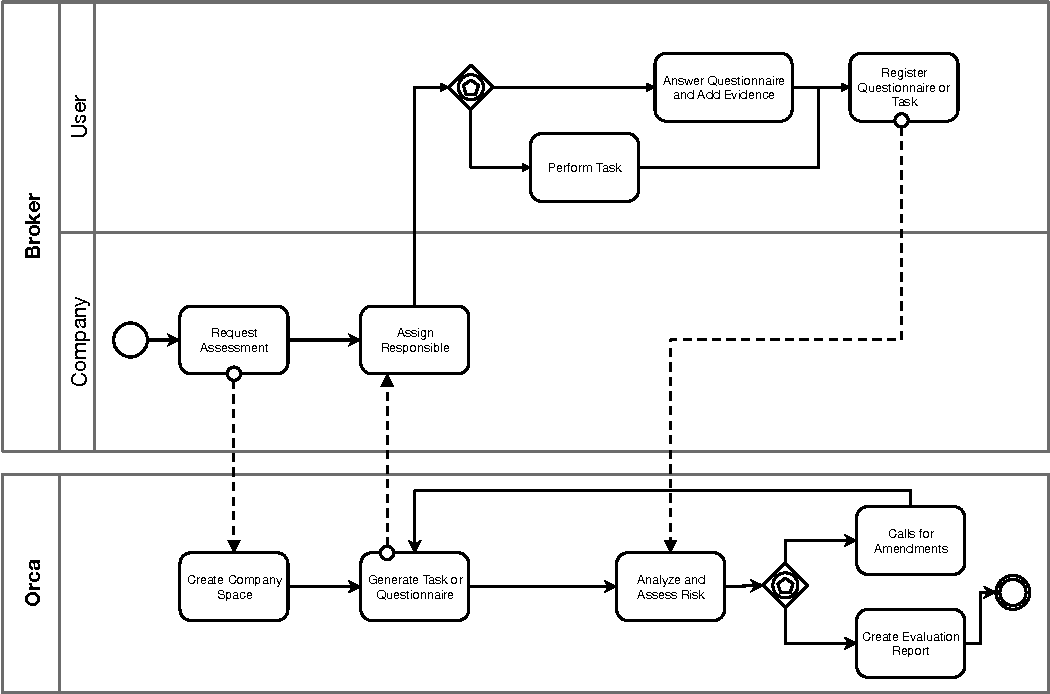
\includegraphics[width=0.6\textwidth]{./figures/BPMN_GCP.pdf}
\caption{BPMN model for \FlyingPig.\label{fig:BPMNmodel}}
\end{figure*}

Once tasks have been completed, they are stored and analyzed to generate a list of non-compliant situations, associated to their corresponding \textit{calls for amendment} (if needed) or a report specifying a compliance level, incidents and a risk map.
During the process of analyzing a questionnaire, the answers to some questions may trigger the generation of additional questionnaires or amendments, that will be scheduled as new tasks.
Business processes also have rules and constraints to define their non-functional requirements (NFR):

\begin{compactenum}
\item An acknowledgement is due in less than 30 seconds after registering a task or demand for assessment.
\item The system should be able to deal with, at least, 200 users.
\item If the number of requests exceeds 200, \FlyingPig\ should implement a load balance strategy for processing the requests.
\item The privileges of the Channel-Broker must be verified \textit{before} the execution of the actions associated to the \textsf{designate user in charge} $\pi$-use case.
\item The privileges of users must be verified \textit{before} the execution of the actions associated to the \textsf{answer questionnaire and add evidences} $\pi$-use case.
\item All questionnaires need to be fully answered in order to consider a task as completed.
\item There is a time limit (in days) for amendments required by the system.
\end{compactenum}

%. . - -. . - -. . - -. . - -. . - -. . - -. . - -. . - -. . - -. . - -. . - -. . - -. . - -. . - -. . - -. . - -. . - -. . - -. . - -. . - -. . - -. . - -. . - -. . - -. . - -. . - -
\subsection{Platform-Independent Models (PIM)}
%. . - -. . - -. . - -. . - -. . - -. . - -. . - -. . - -. . - -. . - -. . - -. . - -. . - -. . - -. . - -. . - -. . - -. . - -. . - -. . - -. . - -. . - -. . - -. . - -. . - -. . - -

%In Section~\ref{sec:modelingWithPISODM} we defined three models at the PIM level.
The \pisodm models of the PIM level  for the \FlyingPig\ scenario are presented next.




\subsubsection{$\pi$-UseCase Model for \FlyingPig}

The $\pi$-UseCase model shown in Figure~\ref{fig:piUseCaseModel} describes the features and constraints of the \FlyingPig\ application.
In this model, three actors are identified: \textit{Company}, \textit{User} and \textit {Broker} represented as stick figures.
Company is the actor requesting a risk evaluation as a Broker is  responsible for coordinating  the evaluation process, assigning users to tasks as well as delegating tasks.
A User is an actor who answers questionnaires according to the current situation  of the Company.
The User also produces evidence to support facts and performs the necessary amendments to improve the results of the risk assessment.
Each actor is associated to $\pi$-UseCases (white ovals in Fig.~\ref{fig:piUseCaseModel})
that describe the main functionality of the system.
The $\pi$-UseCase model for \FlyingPig\ defines six $\pi$-UseCases.
%%
Each $\pi$-UseCase may be associated to (non-functional) constraints (coloured ovals in Fig.~\ref{fig:piUseCaseModel}).
Three types of constraints are defined: \textit{value}, \textit{business} or \textit{exceptional behavior}.
Constraints are identified by the word $<<$\textsf{constraint}$>>$ followed by its type.

\begin{figure*}[h]
\centering
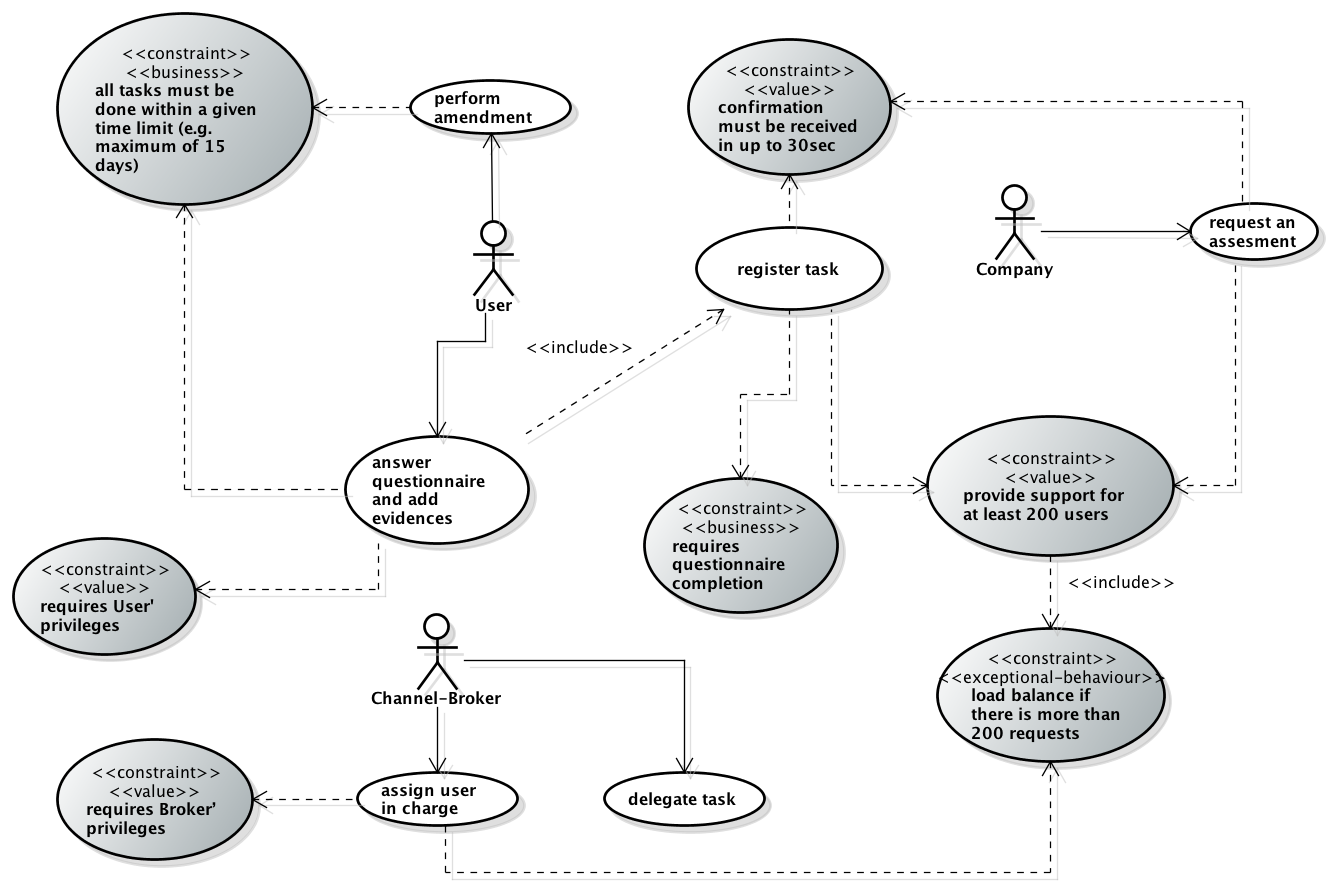
\includegraphics[width=0.55\textwidth]{./figures/UseCaseGeneral.png}
\caption{$\pi$-UseCase model for \FlyingPig.\label{fig:piUseCaseModel}}
\end{figure*}

\subsubsection{$\pi$-ServiceProcess Model for \FlyingPig}

The $\pi$-ServiceProcess model presents the workflow for \FlyingPig (Figure~\ref{fig:PiServiceProcessModel}).
Actions in this model were obtained by applying the $\pi$-use case transformation rules.
The \textsf{Company}, \textsf{Broker-Channel} and \textsf{User} actors are transformed into lanes that represent the business collaborators.
Use cases are transformed into \textit{actions} and are represented by white boxes.
The restrictions associated to  $\pi$-use cases are transformed into \textit{assertions} (represented by colored boxes) and may be decorated with pre- and post-conditions.
We can see that this model refines the concepts defined in the $\pi$-UseCase model.
The assertions specify those non-functional requirements, as they are seen by the actors.
The next step in the development is to add these assertions to the models that specify the \FlyingPig\ system.

\begin{figure*}[h]
\centering
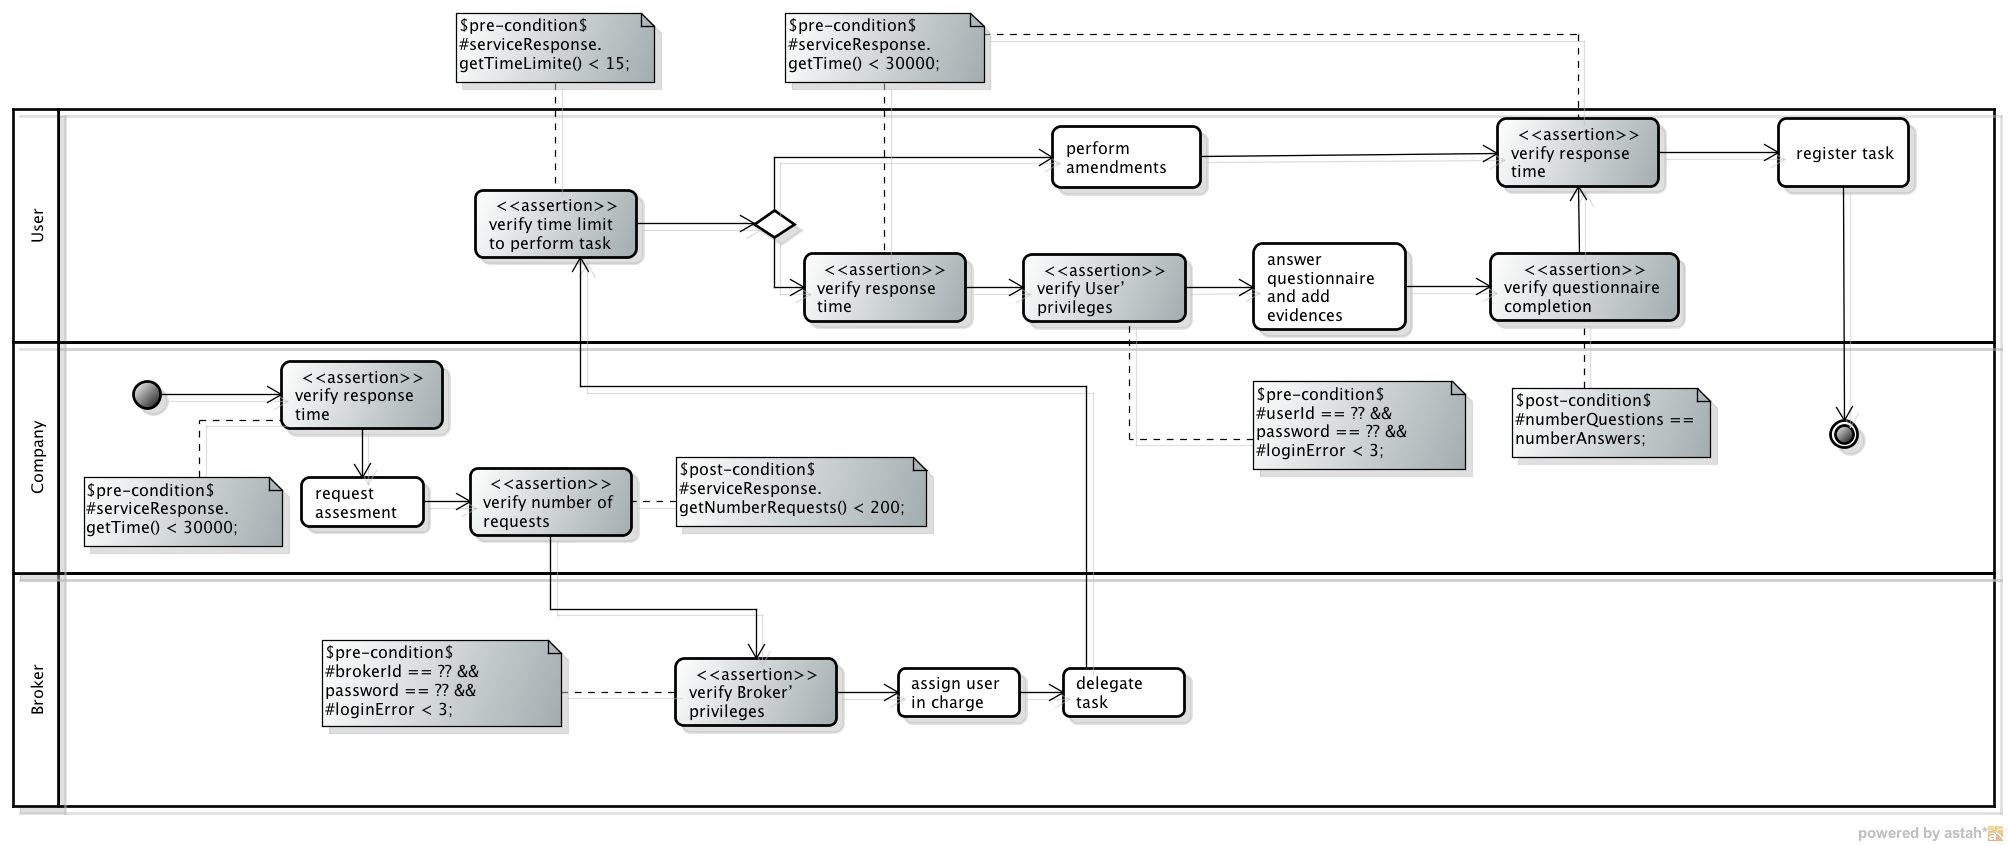
\includegraphics[width=1.0\textwidth]{./figures/ServiceProcessGeneralCut.png}
\caption{$\pi$-ServiceProcess model for \FlyingPig.\label{fig:PiServiceProcessModel}}
\end{figure*}


\subsubsection{$\pi$-ServiceComposition Model for \FlyingPig}

The model in Figure~\ref{fig:PiServiceCompositionModel}
shows  the services that provide the functions of \FlyingPig.
The assertions in Figure~\ref{fig:PiServiceProcessModel} are implemented as \textit{policies}.
These policies express the pre- and post-conditions of the previous model, being  associated to the actions of the system.

\begin{figure*}[h]
\centering
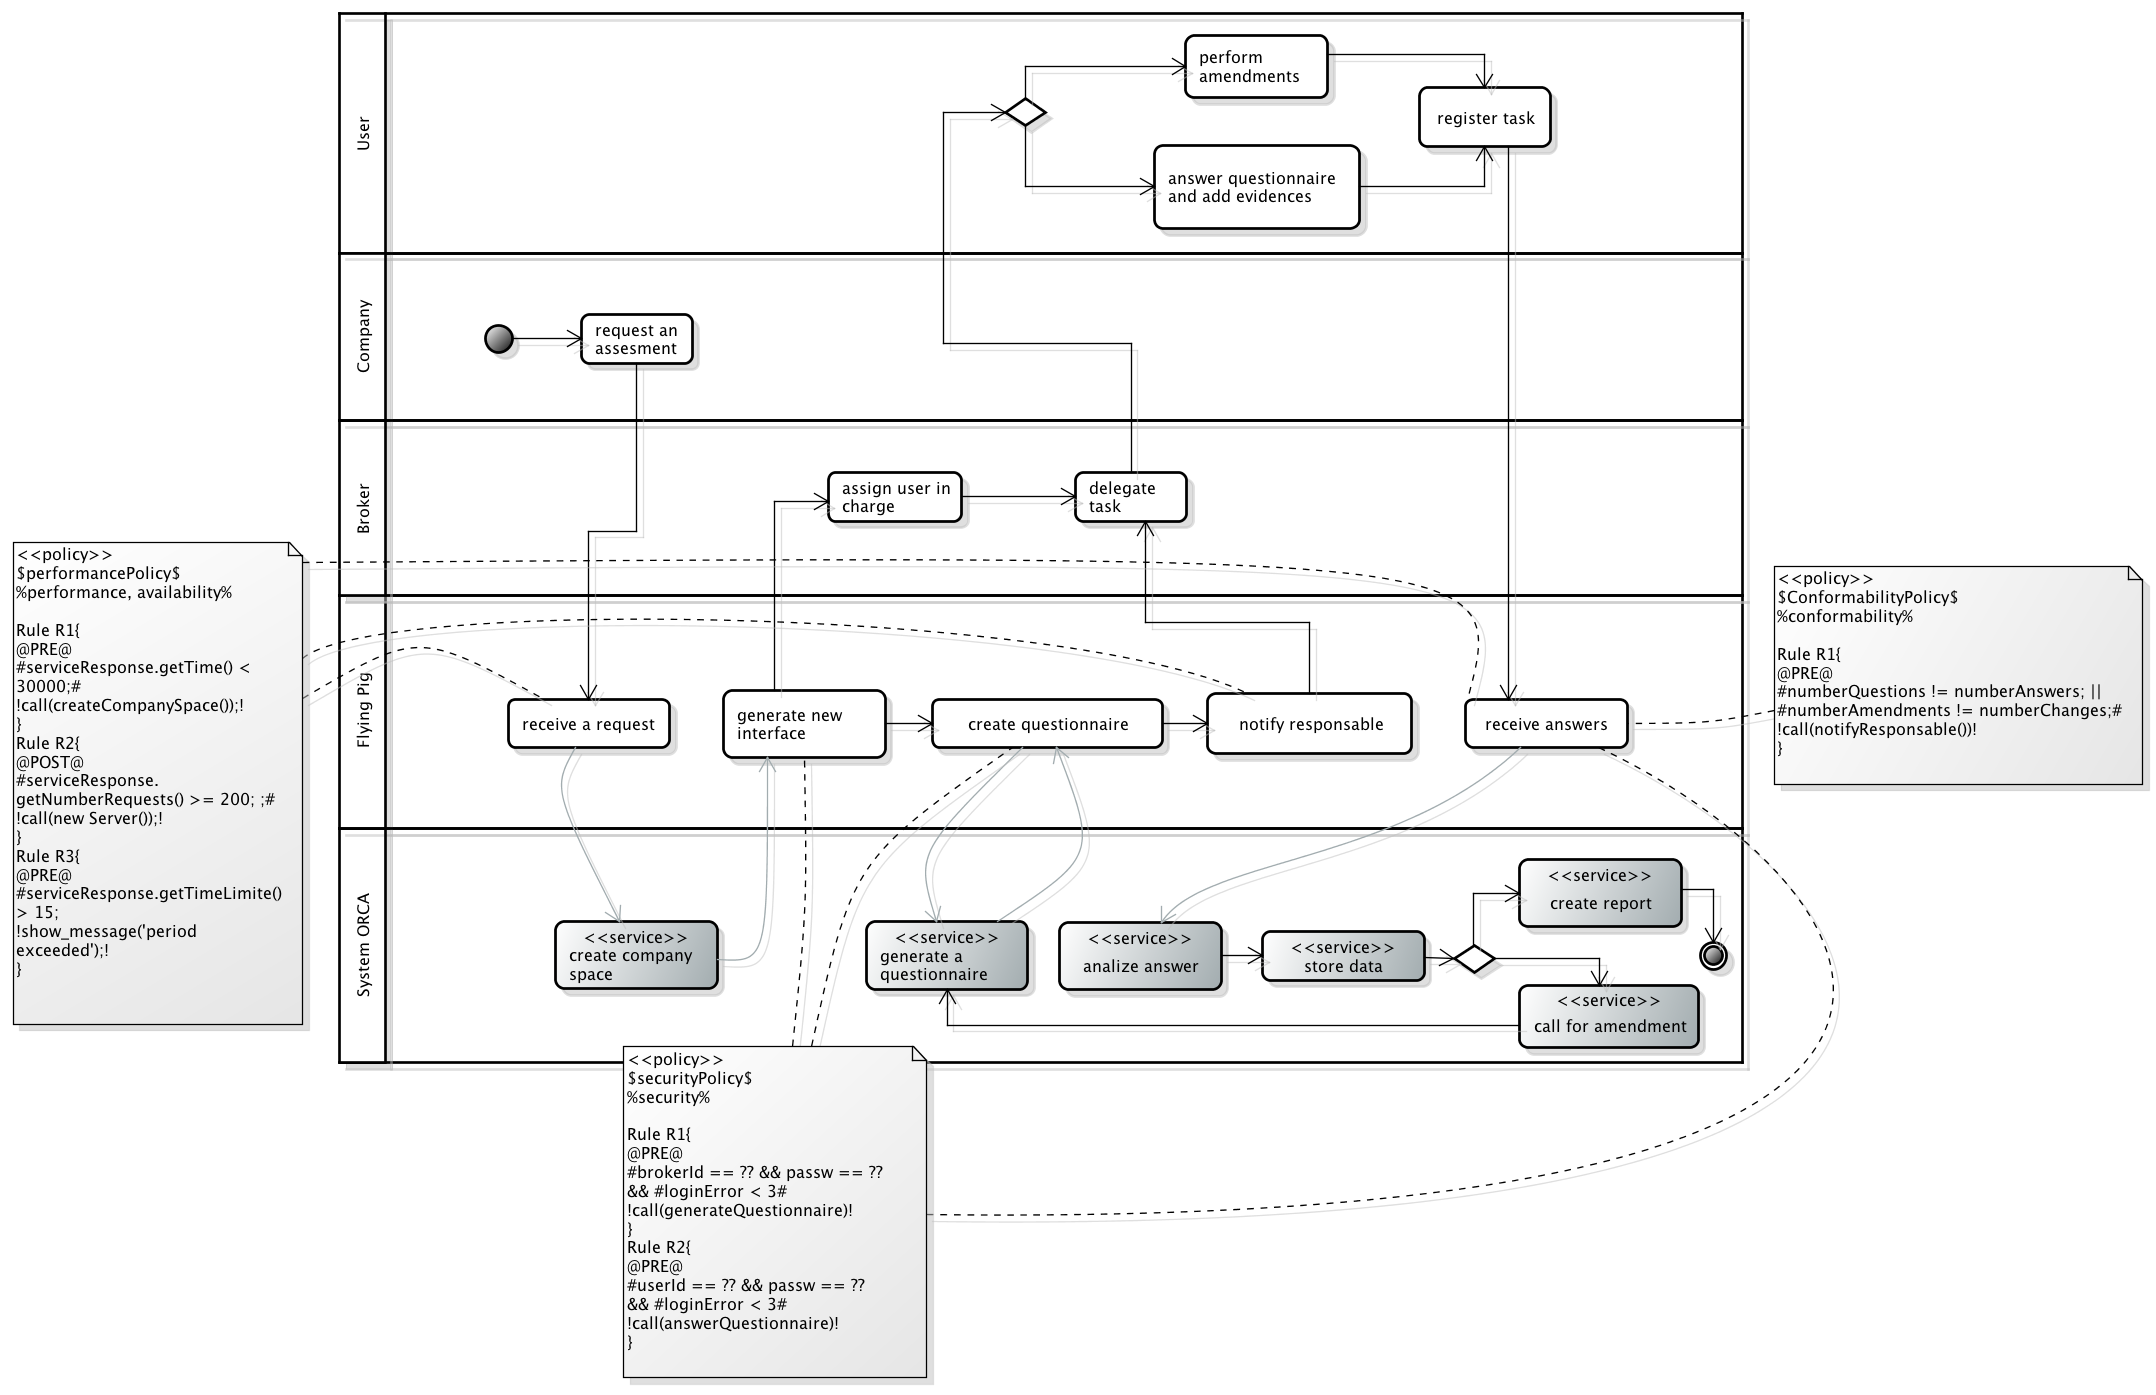
\includegraphics[width=1.0\textwidth]{./figures/ServiceCompositionGeneralCut}
\caption{$\pi$-ServiceComposition model for \FlyingPig.\label{fig:PiServiceCompositionModel}}
\end{figure*}


%. . - -. . - -. . - -. . - -. . - -. . - -. . - -. . - -. . - -. . - -. . - -. . - -. . - -. . - -. . - -. . - -. . - -. . - -. . - -. . - -. . - -. . - -. . - -. . - -. . - -. . - -
%\subsection{Platform-Specific Model (PSM)}
%. . - -. . - -. . - -. . - -. . - -. . - -. . - -. . - -. . - -. . - -. . - -. . - -. . - -. . - -. . - -. . - -. . - -. . - -. . - -. . - -. . - -. . - -. . - -. . - -. . - -. . - -
\subsubsection{$\pi$-PEWS Model for \FlyingPig}

The  PSM of our case study is given in Figure~\ref{fig:piPEWSFlyingPig}. This model is obtained by transforming the $\pi$-service composition model into a workflow.
Note that this workflow is implemented by using  BPEL constructors~\cite{BPEL} and \textit{policy} notions.

\begin{figure*}[h]
\begin{scriptsize}
\begin{verbatim}
//Namespaces specify service URI
namespace orca = www.orca.mx/service.wsdl
//Operations
alias createCompanySpace = portType/createCompanySpace in orca
alias generateQuestionnaire = portType/generateQuestionnaire in orca
alias analizeAnswer = portType/analizeAnswer in orca
alias storeData = portType/storeData in orca
alias createReport = portType/createReport in orca
alias callForAmendments = portType/callForAmendments in orca
//Services
service receiveRequest(R, Id) = createCompanySpace(R, Id)
service generateNewInterface(Id, NULL) = ...
service createQuestionnaire(Id, Q) = generateQuestionnaire(Id, Q)
service notifyResponsable((Id, Q); NULL) = ...
service receiveAnswers((Id, T); P) =
	analizeAnswer((Id, T), NULL) . storeData((Id, T), NULL) . 
	((createReport(Id, P) . return(P)) + (callForAmendments(Id,T) . return(NULL)))
//Workflow
receiveRequest(R, Id)
|| (generateNewInterface(Id, NULL)
 . createQuestionnaire(Id, Q) . notifyResponsable((Id, Q); NULL))
|| (receiveAnswers((Id, T); P) . [P != NULL] STOP)*	
\end{verbatim}
\caption{$\pi$-PEWS Model for \FlyingPig.}\label{fig:piPEWSFlyingPig}
\end{scriptsize}
\end{figure*}



\subsection{Lessons Learned}

Through the example we underlined that every application implements functional aspects that describe its application logic.
Recall that an application logic refers to routines that perform the activities to reach the application objective.
Also there are non functional properties derived from NFR. They refer to strategies to be considered for the application execution like: security, isolation, adaptability, atomicity, and more.
These non functional properties must be ensured at execution time, and they are not completely defined within the application logic.
%
The challenge is to define them and to associate them with the application logic considering that different to existing solutions that suppose that it is possible to access the execution stat of all the components  of an application and that the application has complete control on them, in the case for service oriented applications  the components are autonomous services
API does not necessarily export information about methods dependency (e.g., in the REST protocol);
they do not share their state (stateless).

Given a set of services with their exported methods, building service-based applications may consist on expressing an application logic as a service composition.
During this task, we must ensure the compliance between the specification and the resulting application.
Software engineering methods (e.g., \cite{2,decastro1,PapazoglouH06}) can help to ensure this compliance, particularly when information systems include several sometimes complex business processes calling Web services or legacy applications exported as services.

As WS-* and similar approaches, our work enables the specification and programming of crosscutting aspects (i.e., atomicity, security, exception handling, persistence).
In contrast to these approaches, we specify policies for a services composition in an orthogonal way. Besides, these approaches suppose that non-functional properties are implemented according a the knowledge that a programmer has of a specific application requirements but they are not derived in a methodological way, leading to ad-hoc solutions that can be difficult to reuse. In our approach,  the policies defined for a given application  can be reused and/or specialized for another one with the same requirements or that uses services that impose the same constraints. 


\section{Conclusions and Future Work}\label{sec:conclusions}
We presented \pisodm, a model-driven method for designing and developing reliable service-based applications.
\pisodm extends a previously defined method (called SOD-M) to include Non-Functional Requirements.
These requirements are taken into account from the early stages of the software development process.
Non-functional constraints are related to business rules associated to the behavior of the application and, in the case of service-based applications, they are also concerned with constraints imposed by the services.
%%
Our method includes two CIM-level models, three PIM-level models and one PSM-level model.
We implemented the meta-models on the Eclipse platform and we validated the approach by using an industrially inspired use case.

Our case study was developed together with our industrial partner GCP Global to demonstrate the applicability of \pisodm.
The Company is using \pisodm for the development of their product.
The case study presented is a simplified version of their application. 

\bibliographystyle{plain}
\bibliography{biblio}

\end{document}



